\documentclass[letterpaper, 12pt]{article}
% \usepackage[showframe, margin=1in, top=0.25in, bottom=0.25in, includeheadfoot, headheight=0.5in]{geometry}
\usepackage[margin=1in, top=0.25in, bottom=0.25in, includeheadfoot, headheight=0.5in]{geometry}

\AddToHook{cmd/section/before}{\clearpage}

\usepackage[table]{xcolor}
\colorlet{listingback}{gray!20}
\definecolor{headingcolor}{RGB}{110,34,54}

\usepackage{fancyhdr}
\renewcommand{\sectionmark}[1]{\markboth{#1}{#1}}

% Used to detect whether a section is an appendix to print the right thing in the footer
\usepackage{etoolbox}
\newtoggle{inappendix}
\pretocmd{\appendix}{\clearpage\toggletrue{inappendix}}{}{}

% Save standard definitions for head and foot rules (lines separating header and footer from text)
\let\HeadRule\headrule
\let\FootRule\footrule
% Add color to the standard definitions
\renewcommand{\headrule}{\color{headingcolor}\HeadRule}
\renewcommand{\footrule}{\textcolor{headingcolor}{\FootRule}}

% IMPORTANT: This command should not be called directly. Use \preamble.
% Macro to insert the title page for each lab.
% The argument is the title of the lab.
\newcommand{\inserttitlepage}[1]
{
    \begin{titlepage}
    \centering
    
\includegraphics[scale=0.5]{images/nexus_lab_logo.png}

    \vspace*{\baselineskip}

    \textbf{\Large OpenStack Labs}

    \vspace*{\baselineskip}

    \textbf{\Large #1}
    \vspace*{\fill}
\end{titlepage}
}

% IMPORTANT: This command should not be called directly. Use \preamble.
% Macro to define header and footer for each lab.
% The argument is the title of the lab.
\newcommand{\headfoot}[1]
{
    \fancypagestyle{fancy}
    {
        \fancyhf{}
        \fancyhead[L]{\footnotesize #1}
        \fancyhead[R]{
\includegraphics[height=0.85\headheight]{images/nexus_lab_logo.png}}
        \fancyfoot[L]{%
            \footnotesize%
            \ifnum\value{section}>0%
            \iftoggle{inappendix}{Appendix \thesection: \rightmark}{Section \thesection: \rightmark}%
            \fi}
        \fancyfoot[R]{\footnotesize\thepage}
        \renewcommand{\headrulewidth}{1.5pt}
        \renewcommand{\footrulewidth}{1.5pt}
    }
}

% Macro to insert title page, define header and footer, and insert table of contents and about section for each lab.
% The argument is the title of the lab.
\newcommand{\preamble}[1]
{
    \pagenumbering{roman}
    \inserttitlepage{#1}
    \headfoot{#1}

    % Insert table of contents
    \pagestyle{fancy}
    \tableofcontents
    \clearpage

    \section*{About This Document}
    \label{sec:about_this_document}
    \begin{itemize}
        \item This document was developed by a team at the University of Tennessee at Chattanooga led by Dr. Mengjun Xie
        (\href{mailto:mengjun-xie@utc.edu}{\textbf{mengjun-xie@utc.edu}}).
        \item The development of this document was supported by a National Centers of Academic Excellence in Cybersecurity Grant (\#H98230-20-1-0351), housed at the National Security Agency.
        \item This document is licensed with a Creative Commons Attribution 4.0 International License.
    \end{itemize}
    \clearpage
}

% Macro to insert the Lab Settings page for each lab. Call after the Introduction and Objectives sections.
\newcommand{\labsettings}
{
    \section*{Lab Settings}
    \label{sec:lab_settings}
    \addcontentsline{toc}{section}{\nameref{sec:lab_settings}}
    The information in the table below will be needed in order to complete the lab.
    The task sections below provide details on the use of this information.
    \begin{table*}[htbp]
        \centering
        \begin{tabular}{|c|c|c|c|}
            \hline
            \rowcolor{gray!20} \textbf{Virtual Machine} & \textbf{IP Address} & \textbf{Account} & \textbf{Password} \\
            \hline
            \multirow{2}{*}{\texttt{workstation}} & \multirow[t]{2}{*}{\texttt{ens3: 192.168.1.21}}  & \multirow{2}{*}{\texttt{ubuntu}} & \multirow{2}{*}{\texttt{ubuntu}} \\
                                                  & \multirow[t]{2}{*}{\texttt{ens4: 172.25.250.21}} &                                  &                                  \\
            \hline
            \multirow{2}{*}{\texttt{devstack}}    & \multirow[t]{2}{*}{\texttt{ens3: 192.168.20}}    & \multirow{2}{*}{\texttt{ubuntu}} & \multirow{2}{*}{\texttt{ubuntu}} \\
                                                  & \multirow[t]{2}{*}{\texttt{ens4: 172.25.250.20}} &                                  &                                  \\
            \hline
        \end{tabular}
    \end{table*}
    \clearpage

    % IMPORTANT(lucas): If another frontmatter section ever gets placed after this, this command needs to be moved
    % to the end of that section.
    % I have placed this here and not in each lab purely for convenience and to ensure I don't forget any.
    \pagenumbering{arabic}
}

% Sans-serif font
\renewcommand{\familydefault}{\sfdefault}
\newcommand{\texttildemid}{{\raisebox{0.5ex}{\texttildelow}}}

\usepackage{enumitem}
\renewcommand{\labelenumi}{\textbf{\thesection.\arabic{enumi}.}}

% Try to forbid widows and orphans
\widowpenalty10000
\clubpenalty10000

\usepackage{graphicx}
\usepackage{hyperref}
\hypersetup{colorlinks=true,linkcolor=black,urlcolor={[named] headingcolor}}

\usepackage{sectsty}
\sectionfont{\color{headingcolor}}

% Table of Contents
\usepackage{bookmark}
\usepackage[titles]{tocloft}
\usepackage[title]{appendix}
\renewcommand{\cfttoctitlefont}{\Large\bfseries\color{headingcolor}}
\renewcommand{\cftsecfont}{\normalfont\normalsize}
\renewcommand{\cftsecpagefont}{\normalfont\normalsize}
\renewcommand{\cftdotsep}{0} % Make dots small and close together
\renewcommand{\cftsecleader}{\cftdotfill{\cftdotsep}} % Add dots after section titles
% Make dots go all the way to the page number
\renewcommand{\cftsecfillnum}[1]{{\cftsecleader}\nobreak{\cftsecpagefont #1}\cftsecafterpnum\par}

\usepackage{multirow}
\setlength{\tabcolsep}{16pt}
\renewcommand{\arraystretch}{1.1}

% For nice-looking boxes
\usepackage[most]{tcolorbox}
\usepackage{listings}
\usepackage{lstautogobble}
\lstset{
  frame=none,
  language=Bash,
  showstringspaces=false,
  basicstyle={\linespread{1.1}\footnotesize\ttfamily\selectfont},
  numbers=none,
  breaklines=true,
  breakatwhitespace=true,
  tabsize=3,
  columns=fullflexible,
  keepspaces=true,
  escapeinside={(*@}{@*)},
  literate={~}{{\texttildemid}}{1}
           {\#}{\#}{1},
  autogobble=true
}

\tcolorboxenvironment{lstlisting}
{
    spartan,
    colframe=gray!50,
    boxsep=0mm,
    left=1mm,
    right=1mm,
    top=-1mm,
    bottom=-1mm,
    colback=gray!20
}

% Hacky solution for now, would like to have just one environment and make several tcolorboxes by passing different
% colors as parameters, but that is giving errors
\makeatletter
\tcbset{
  note/.style={%
        enhanced,
        breakable,
        colback=blue!10!white,
        colframe=blue!80!white,
        attach boxed title to top left={yshift*=-\tcboxedtitleheight},
        title={#1},
        boxed title size=title,
        boxed title style={%
            sharp corners,
            rounded corners=northwest,
            colback=tcbcolframe,
            boxrule=0pt,
        },
        underlay boxed title={%
            \path[fill=tcbcolframe] (title.south west)--(title.south east)
                to[out=0, in=180] ([xshift=5mm]title.east)--
                (title.center-|frame.east)
                [rounded corners=\kvtcb@arc] |-
                (frame.north) -| cycle;
        },
    }
}
\makeatother

\makeatletter
\tcbset{
    stop/.style={%
        enhanced,
        breakable,
        colback=white,
        colback=red!10!white,
        colframe=red!80!white,
        attach boxed title to top left={yshift*=-\tcboxedtitleheight},
        title={#1},
        boxed title size=title,
        boxed title style={%
            sharp corners,
            rounded corners=northwest,
            colback=tcbcolframe,
            boxrule=0pt,
        },
        underlay boxed title={%
            \path[fill=tcbcolframe] (title.south west)--(title.south east)
                to[out=0, in=180] ([xshift=5mm]title.east)--
                (title.center-|frame.east)
                [rounded corners=\kvtcb@arc] |-
                (frame.north) -| cycle;
        },
    }
}
\makeatother

\makeatletter
\tcbset{
    tip/.style={%
        enhanced,
        breakable,
        colback=white,
        colback=green!10,
        colframe=green!70!black,
        attach boxed title to top left={yshift*=-\tcboxedtitleheight},
        fonttitle=\bfseries,
        title={#1},
        boxed title size=title,
        boxed title style={%
            sharp corners,
            rounded corners=northwest,
            colback=tcbcolframe,
            boxrule=0pt,
        },
        underlay boxed title={%
            \path[fill=tcbcolframe] (title.south west)--(title.south east)
                to[out=0, in=180] ([xshift=5mm]title.east)--
                (title.center-|frame.east)
                [rounded corners=\kvtcb@arc] |-
                (frame.north) -| cycle;
        },
    }
}
\makeatother

% The commands below define environments for colored boxes. They are used like
% \begin{notebox}
% ...
% \end{notebox}
\newtcolorbox{notebox}{note={Note}}
\newtcolorbox{stopbox}{stop={Stop}}
\newtcolorbox{tipbox}{tip={Tip}}

\begin{document}
\preamble{Lab 04: Deploying an External Network}

\section*{Introduction}\label{sec:introduction}
\addcontentsline{toc}{section}{\nameref{sec:introduction}}
Up to this point, everything you have worked on has been local to the OpenStack environment.
In this lab, you will manage external networks, routers, and floating IP addresses to give OpenStack instances and networks external connectivity.
These resources will come together in the next lab to allow OpenStack instances to provide services outside the OpenStack cloud and allow you to manage instances from outside the cloud.

\section*{Objectives}\label{sec:objectives}
\addcontentsline{toc}{section}{\nameref{sec:objectives}}
\begin{itemize}[itemsep=0pt]
    \item Create and manage external networks.
    \item Create and manage OpenStack routers.
    \item Create and manage floating IP addresses.
\end{itemize}
\clearpage

\labsettings

%%%%%%%%%%%
% Section 1
%%%%%%%%%%%
\section{Managing External Networks}\label{sec:managing-external-networks}
In this task, you will use the \textit{Horizon Dashboard} and the \textit{OpenStack Unified CLI} to create and configure an external network.
Resources on this network will be accessible to users outside the OpenStack environment.

\begin{enumerate}
    \begin{labstep}
        Log into the \textbf{workstation} machine as the \textbf{ubuntu} user with password \textbf{ubuntu}.

        \begin{center}
            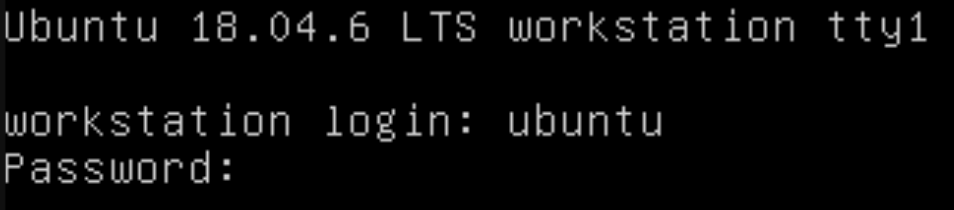
\includegraphics[width=\linewidth]{images/part1/step1.png}
        \end{center}
    \end{labstep}

    \begin{labstep}
        Launch the graphical user interface.
        \begin{lstlisting}
            ubuntu@workstation:~$ startx
        \end{lstlisting}

        \begin{center}
            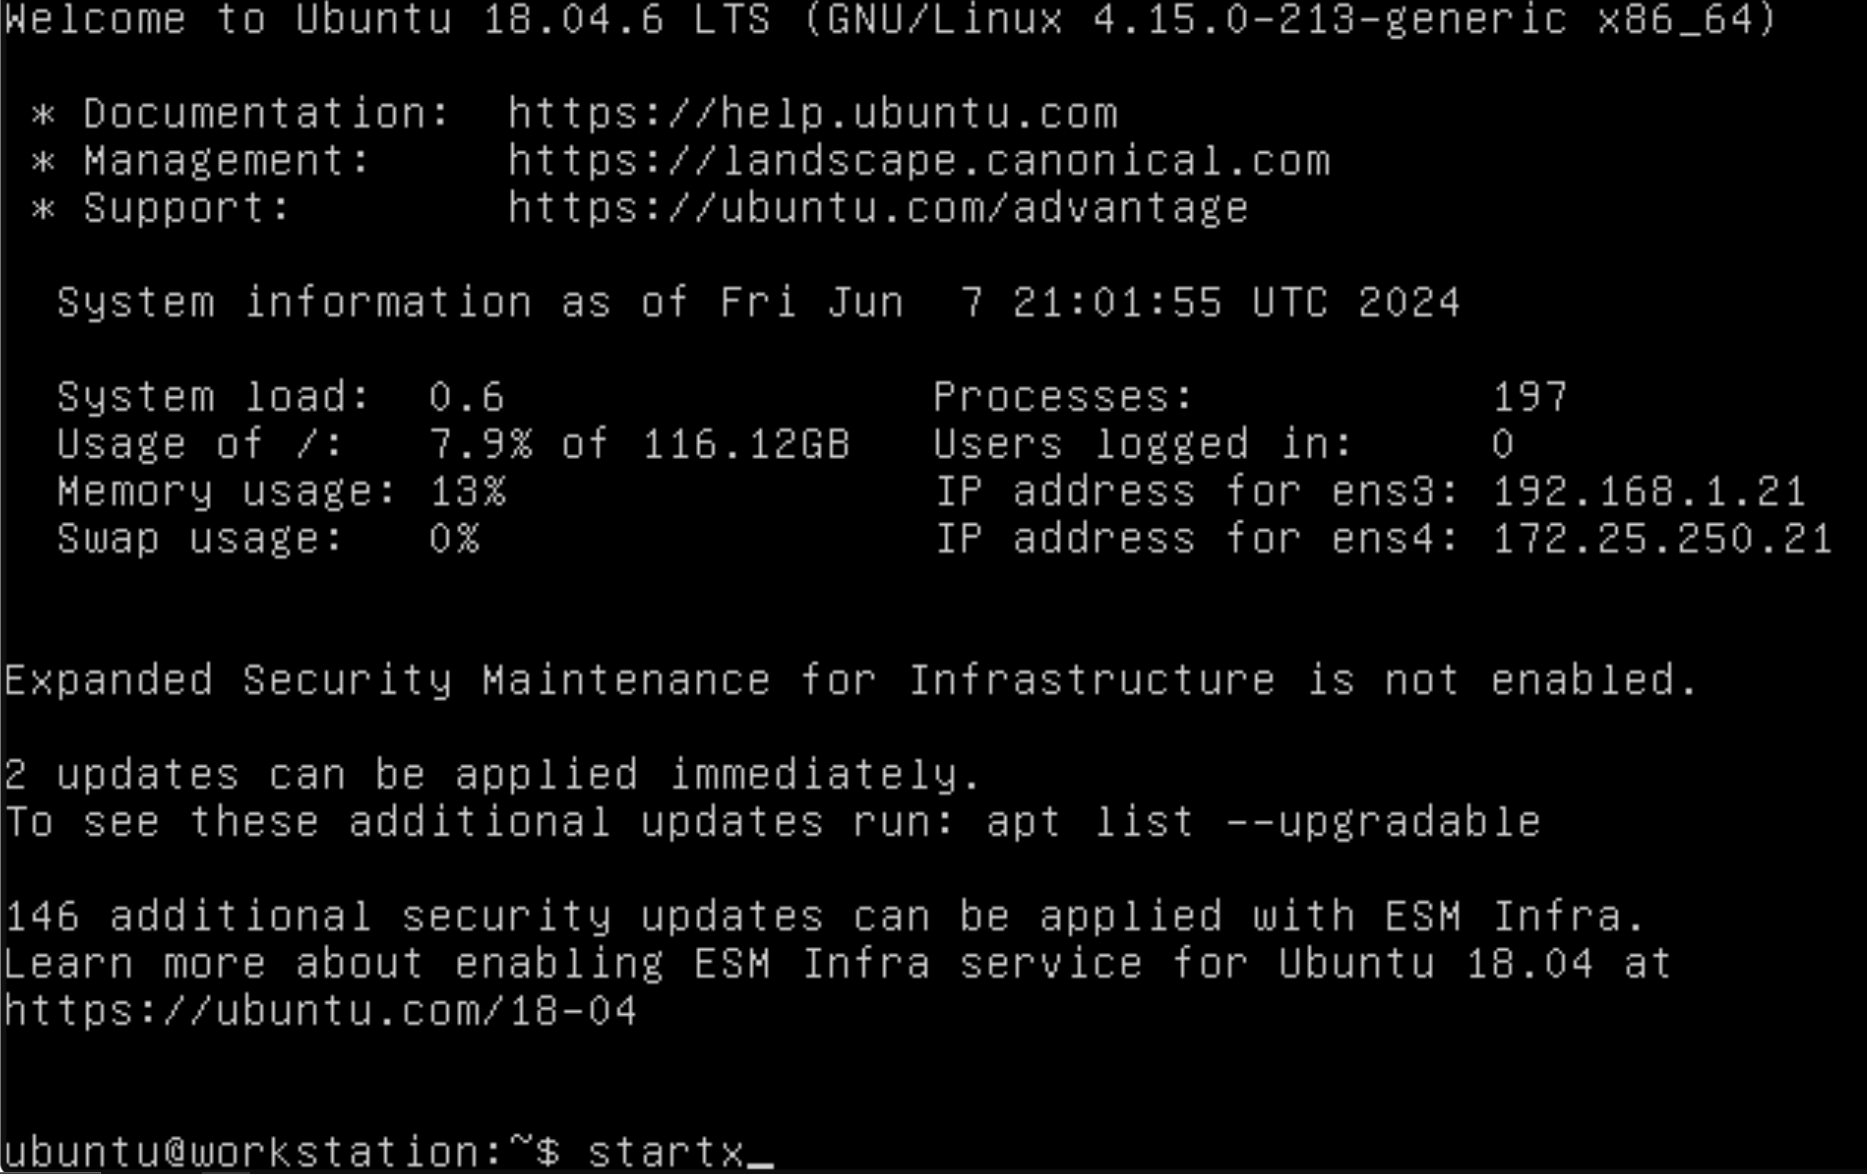
\includegraphics[width=\linewidth]{images/part1/step2.png}
        \end{center}
    \end{labstep}

    \begin{labstep}
        Open the web browser.
        Navigate to \textbf{192.168.1.20} and log in to the dashboard as \textbf{admin} with the password \textbf{secret}.
        In this lab, we will create our own public network and router.
        The \textbf{demo} project already has a default router and public network, so those need to be deleted first.

        \begin{center}
            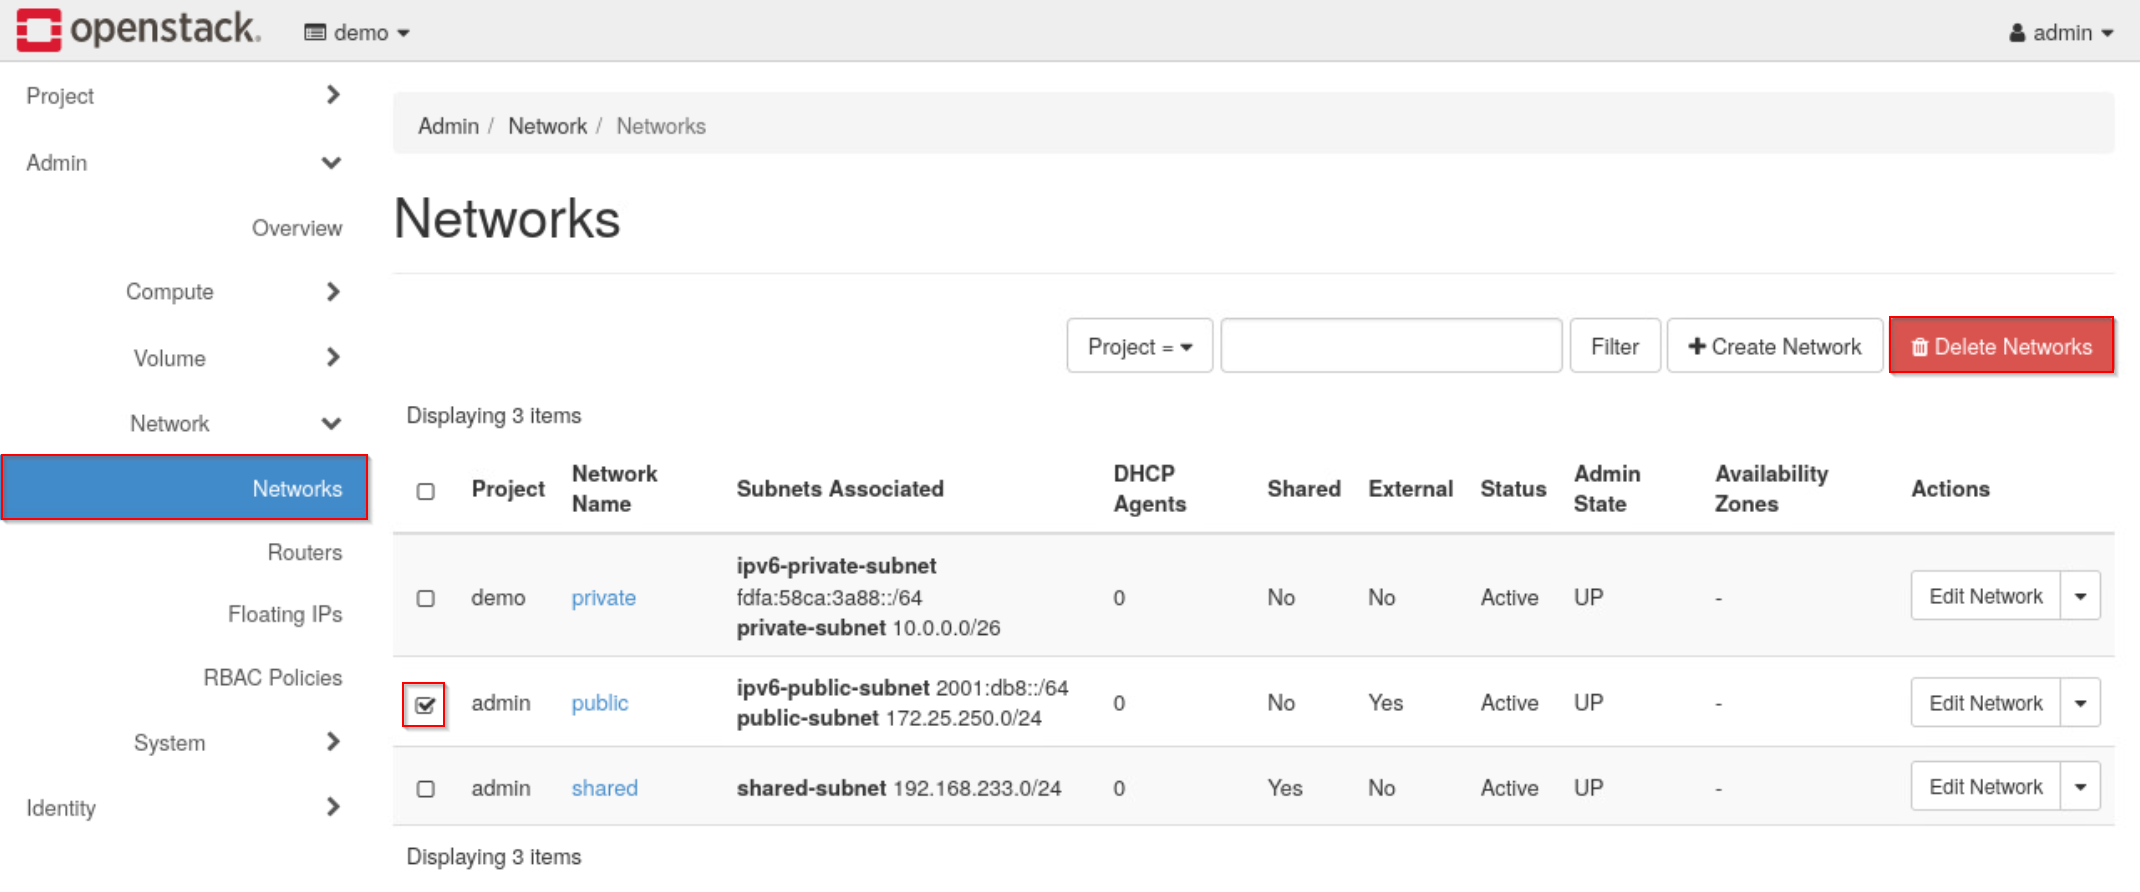
\includegraphics[scale=0.5]{images/part1/step3.png}
        \end{center}
    \end{labstep}

    \begin{labstep}
        Select the \textbf{demo} project.
        Navigate to \textbf{Admin $>$ Network $>$ Routers}.
        Check the box in the same row as \textbf{router1}, then click \textbf{Delete Routers}.

        \begin{center}
            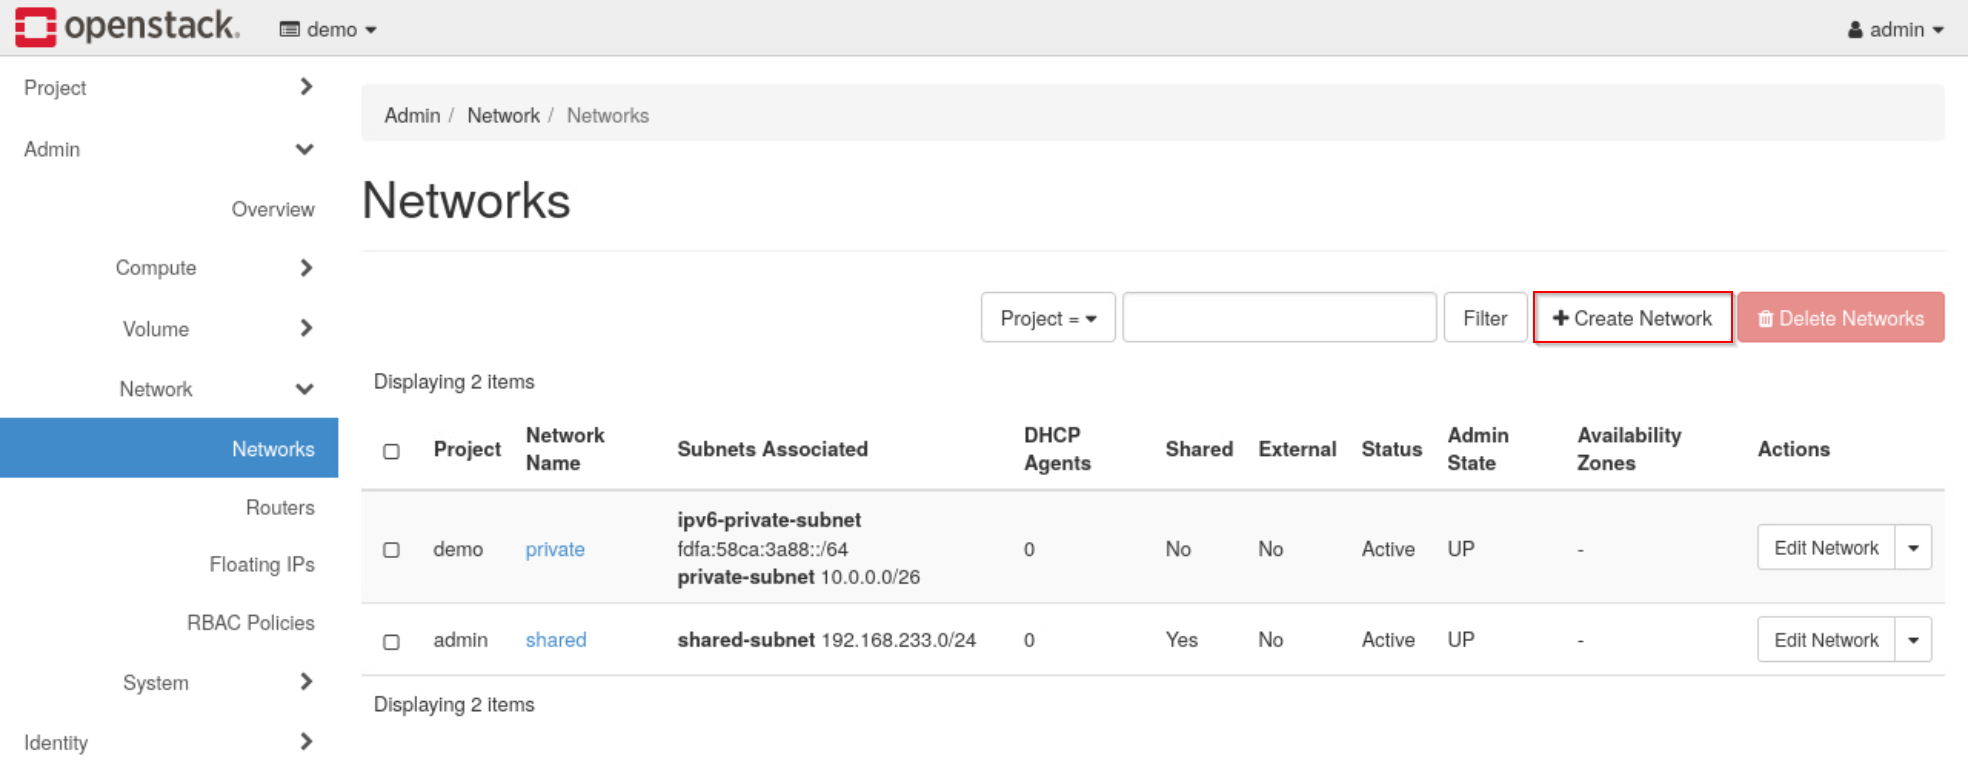
\includegraphics[width=\linewidth]{images/part1/step4.png}
        \end{center}
    \end{labstep}

    \begin{labstep}
        Now, navigate to \textbf{Networks}.
        Check the box in the same row as \textbf{public}, then click
        \textbf{Delete Networks}.

        \begin{center}
            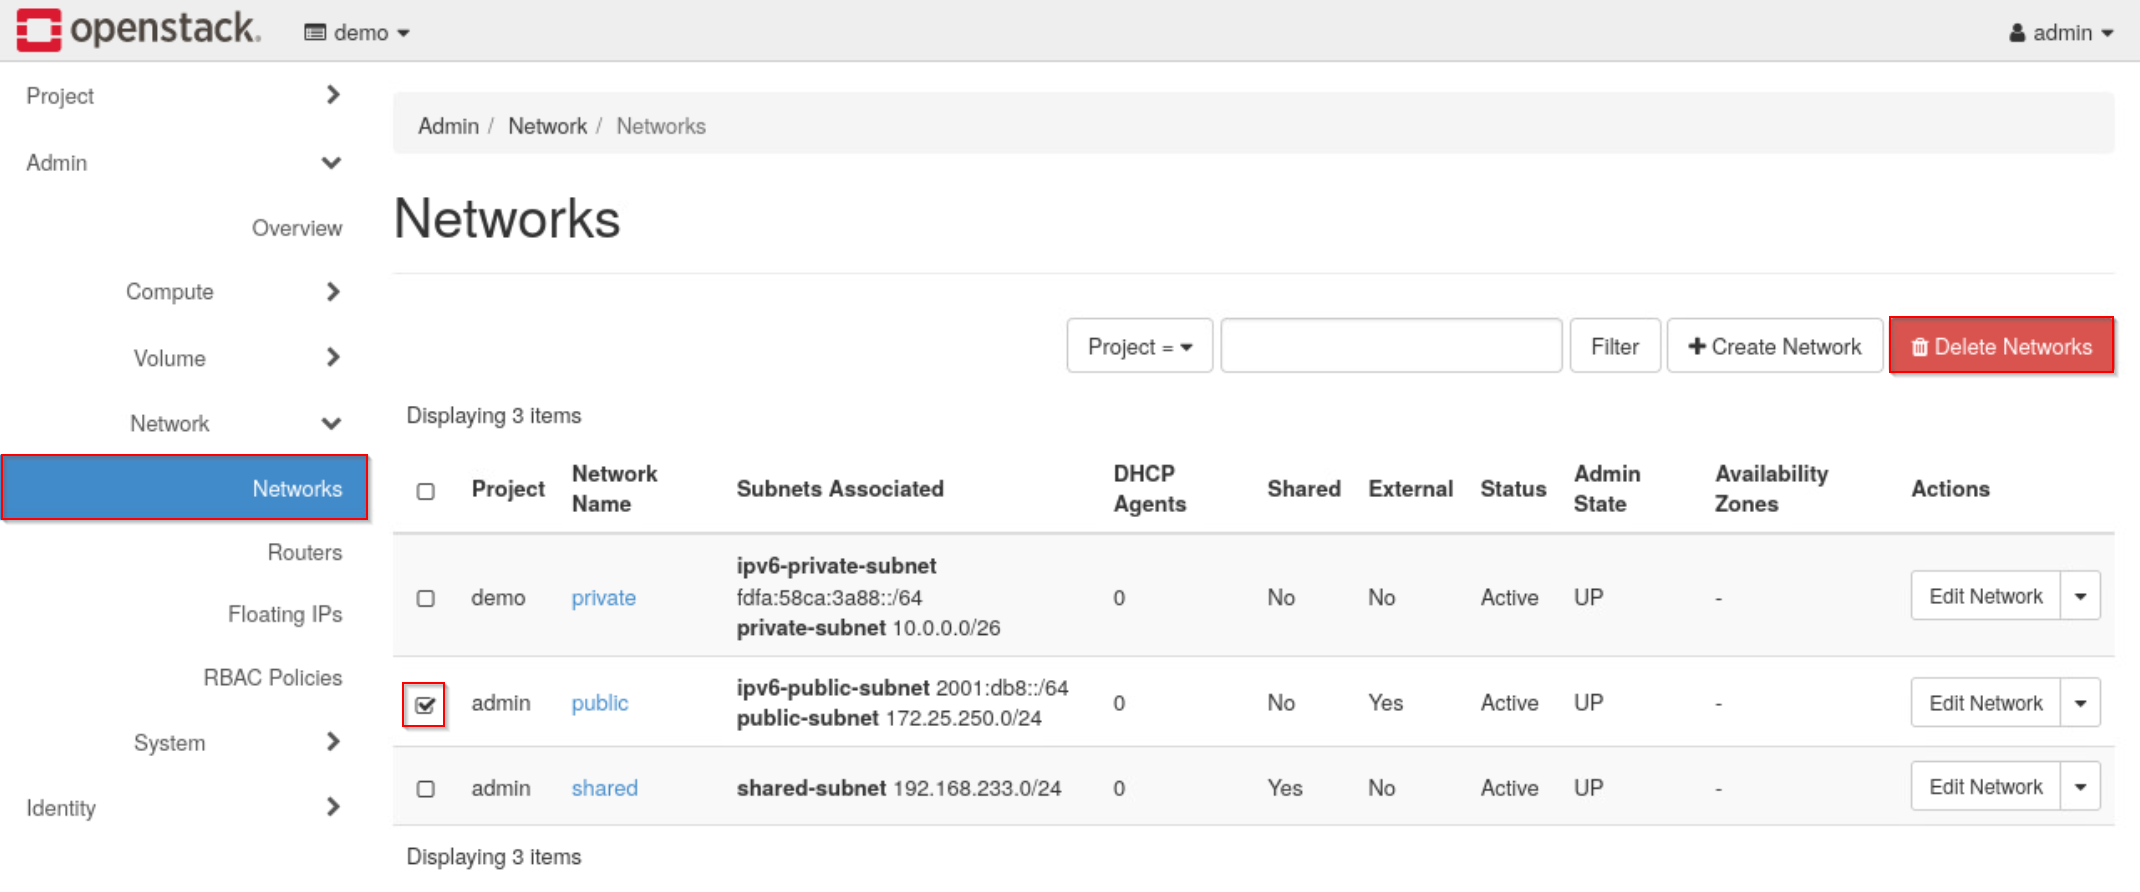
\includegraphics[width=\linewidth]{images/part1/step5.png}
        \end{center}
    \end{labstep}

    \begin{notebox}
        If you try to delete the \textbf{public} network before deleting the router, you will receive an error saying ``one or more ports still exist on the requested network''.
        Therefore, it is necessary to delete any external interfaces (gateways) that exist on routers attached to a network before deleting the network.
        When a router is deleted, all of its ports are automatically deleted.
    \end{notebox}

    \begin{labstep}
        Click \textbf{Create Network}.

        \begin{center}
            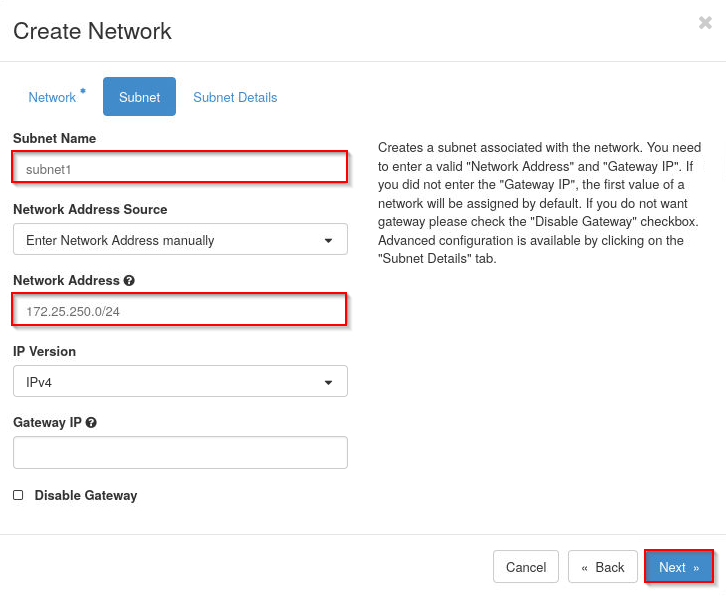
\includegraphics[width=\linewidth]{images/part1/step6.png}
        \end{center}
    \end{labstep}

    \begin{labstep}
        Enter \textbf{extern-net1} in the \textit{Network Name} field.
        Select \textbf{demo} in the \textit{Project} dropdown.
        For \textit{Provider Network Type}, select \textbf{Flat}.
        Enter \textbf{public} into the \textit{Physical Network} field.
        Check the \textit{Shared} and \textit{External Network} check boxes, and ensure the \textit{Create Subnet} check box is checked.
        Click \textbf{Next} to go to the \textit{Subnet} tab.

        \begin{center}
            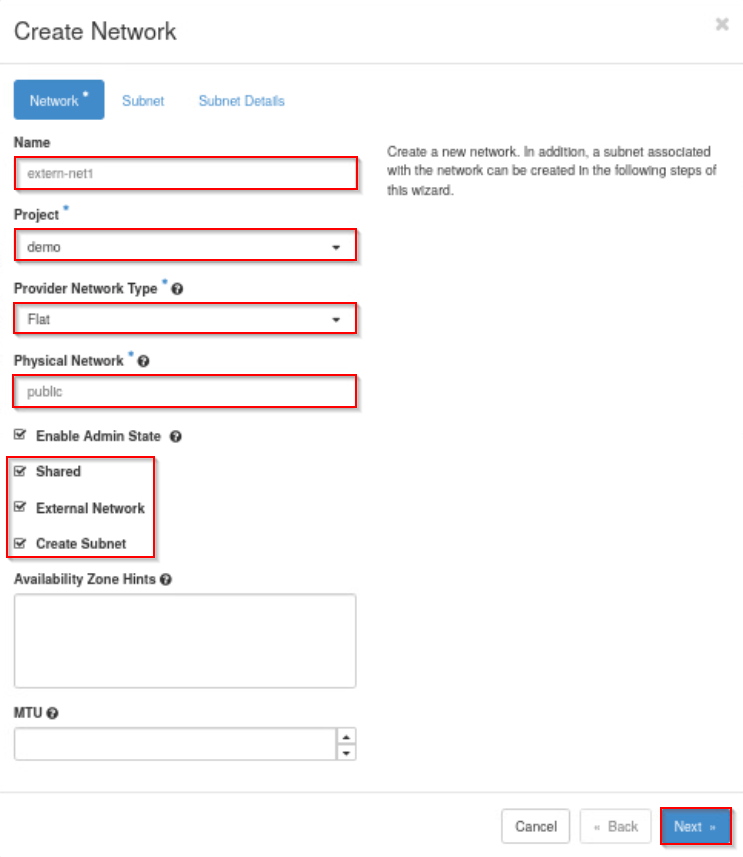
\includegraphics[width=\linewidth]{images/part1/step7.png}
        \end{center}
    \end{labstep}

    \begin{tipbox}
        If your \textbf{Create Network} form looks different, you likely navigated to \textbf{Project $>$ Network $>$ Networks}.
        You can only create external networks from the \textbf{Admin $>$ Network $>$ Networks} tab.
    \end{tipbox}
    \begin{notebox}
        The \textbf{public} physical network you will use in this task is not the same as the \textbf{public} network you just deleted.
        The deleted network was a virtual network built on top of a physical network, and they just happen to have the same name.
        The physical \textbf{public} network still exists because it is a separate resource used by OpenStack for external communication.
    \end{notebox}

    \begin{labstep}
        In the \textit{Subnet} tab, enter \textbf{extern-subnet1} in the \textit{Subnet Name} field, enter \textbf{172.25.250.0/24} in the \textit{Network Address} field, and enter \textbf{172.25.250.254} in the \textit{Gateway IP} field.
        Click \textbf{Next} to go to the \textit{Subnet Details} tab.

        \begin{center}
            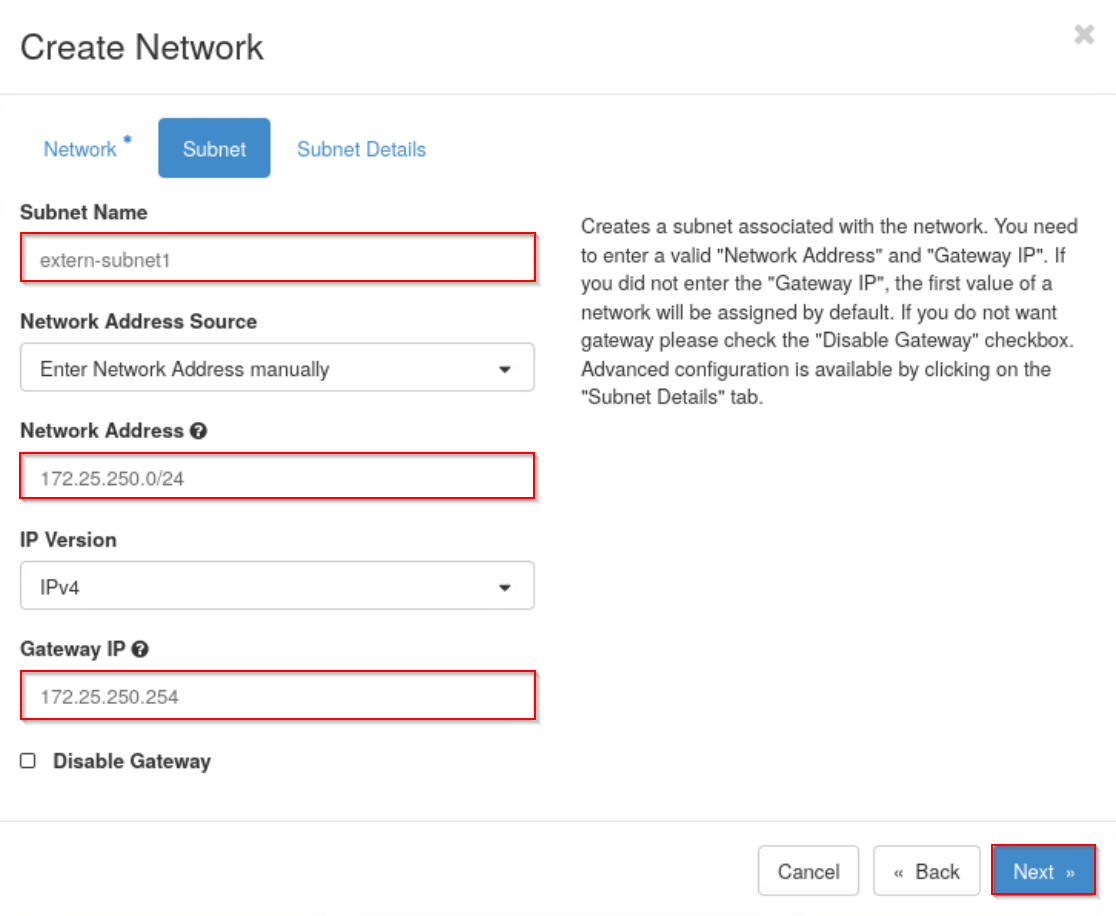
\includegraphics[width=\linewidth]{images/part1/step8.png}
        \end{center}
    \end{labstep}

    \begin{labstep}
        In the \textit{Subnet Details} tab, uncheck the \textit{Enable DHCP} check box since we want to assign static IP addresses on this network.
        Enter \textbf{172.25.250.60,172.25.250.80} in the \textit{Allocation Pools} field so that any IP address allocated for this network will fall in this range of addresses.
        Enter \textbf{172.25.250.254} in the \textit{DNS Name Servers} field.
        Click \textbf{Create} to create the network and subnet.

        \begin{center}
            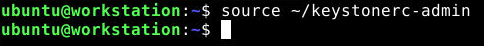
\includegraphics[width=\linewidth]{images/part1/step9.png}
        \end{center}
    \end{labstep}

    \begin{labstep}
        Log out of the \textit{Horizon Dashboard}, and close the web browser.
    \end{labstep}

    \begin{labstep}
        Open a terminal window and source the keystone credentials for the \textbf{admin} user.
        \begin{lstlisting}
            ubuntu@workstation:~$ source ~/keystonerc-admin
        \end{lstlisting}

        \begin{center}
            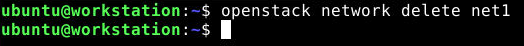
\includegraphics[width=\linewidth]{images/part1/step11.png}
        \end{center}
    \end{labstep}

    \begin{labstep}
        List the available networks.
        \begin{lstlisting}
            [ubuntu@workstation (keystone-admin)]:~$ openstack network list
        \end{lstlisting}

        \begin{center}
            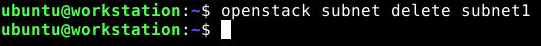
\includegraphics[width=\linewidth]{images/part1/step12.png}
        \end{center}
    \end{labstep}

    \begin{labstep}
        The next set of steps will show how to recreate the external network from the beginning of the lab from the CLI.
        To free up the necessary resources, first delete the \textbf{extern-net1} network.
        This will also delete the \textbf{extern-subnet1} subnet.
        \begin{lstlisting}
            [ubuntu@workstation (keystone-admin)]:~$ openstack network delete extern-net1
        \end{lstlisting}

        \begin{center}
            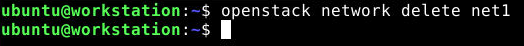
\includegraphics[width=\linewidth]{images/part1/step13.png}
        \end{center}
    \end{labstep}

    \begin{labstep}
        List the networks again to confirm that \textbf{extern-net1} was deleted successfully.
        \begin{lstlisting}
            [ubuntu@workstation (keystone-admin)]:~$ openstack network list
        \end{lstlisting}

        \begin{center}
            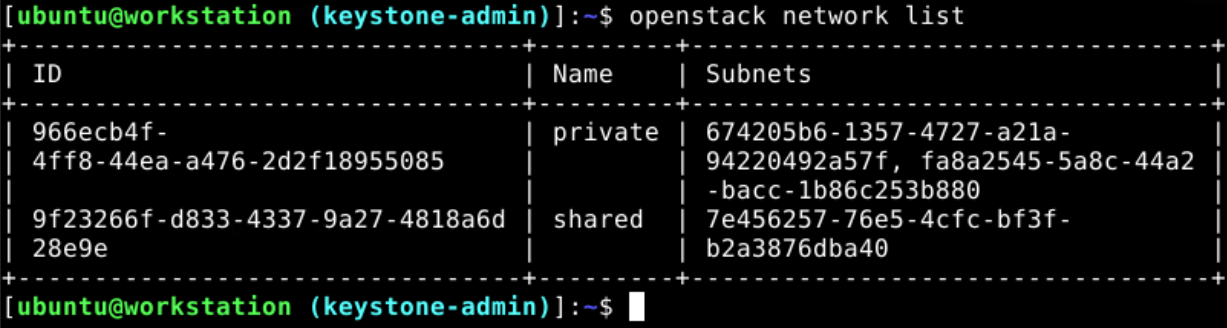
\includegraphics[width=\linewidth]{images/part1/step14.png}
        \end{center}
    \end{labstep}

    \begin{labstep}
        Create an external network named \textbf{extern-net2}.
        Set the network type to \textbf{flat} and the physical network to \textbf{public}.
        Set the network as shared and external.
        \begin{lstlisting}
            [ubuntu@workstation (keystone-admin)]:~$ openstack network create \
            > --external \
            > --share \
            > --provider-network-type flat \
            > --provider-physical-network public \
            > extern-net2
        \end{lstlisting}

        \begin{center}
            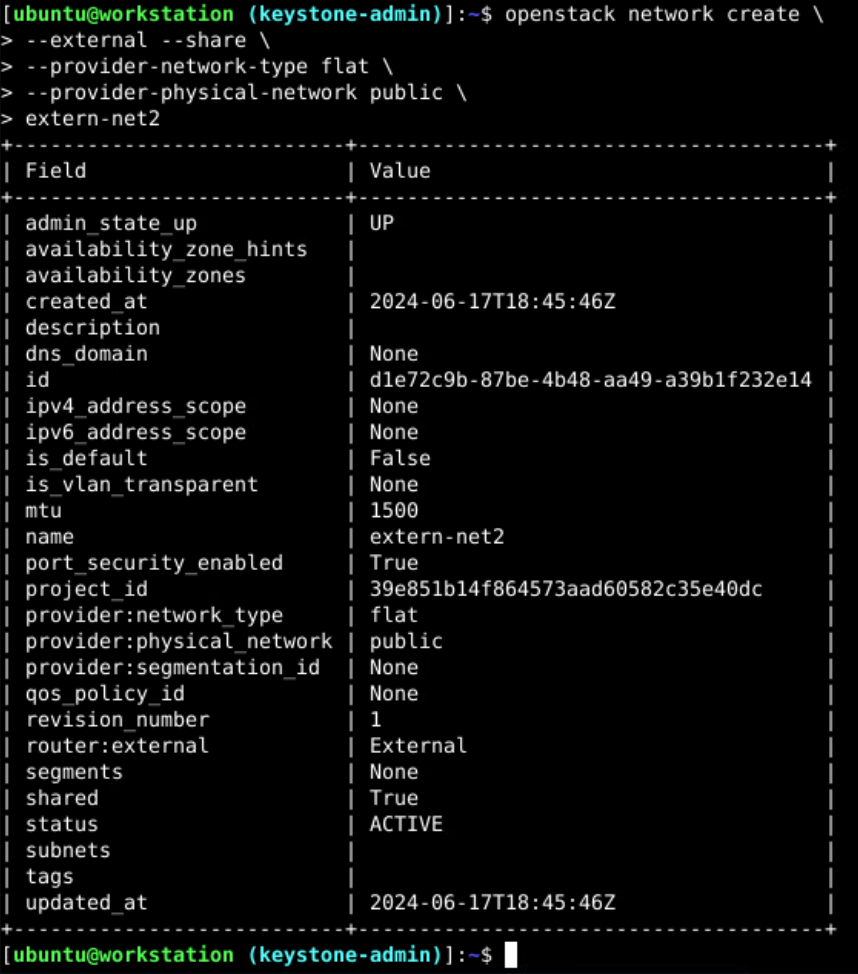
\includegraphics[width=\linewidth]{images/part1/step15.png}
        \end{center}
    \end{labstep}

    \begin{labstep}
        Create a subnet named \textbf{extern-subnet2} in the \textbf{extern-net2} network.
        Give the subnet a range of \textbf{172.25.250.60} to \textbf{172.25.250.80}.
        Disable DHCP services for the subnet and use the address \textbf{172.25.250.254} as the gateway as well as the DNS name server.
        \begin{lstlisting}
            [ubuntu@workstation (keystone-admin)]:~$ openstack subnet create \
            > --subnet-range 172.25.250.0/24 \
            > --no-dhcp \
            > --gateway 172.25.250.254 \
            > --dns-nameserver 172.25.250.254 \
            > --allocation-pool start=172.25.250.60,end=172.25.250.80 \
            > --network extern-net2 \
            > extern-subnet2
        \end{lstlisting}

        \begin{center}
            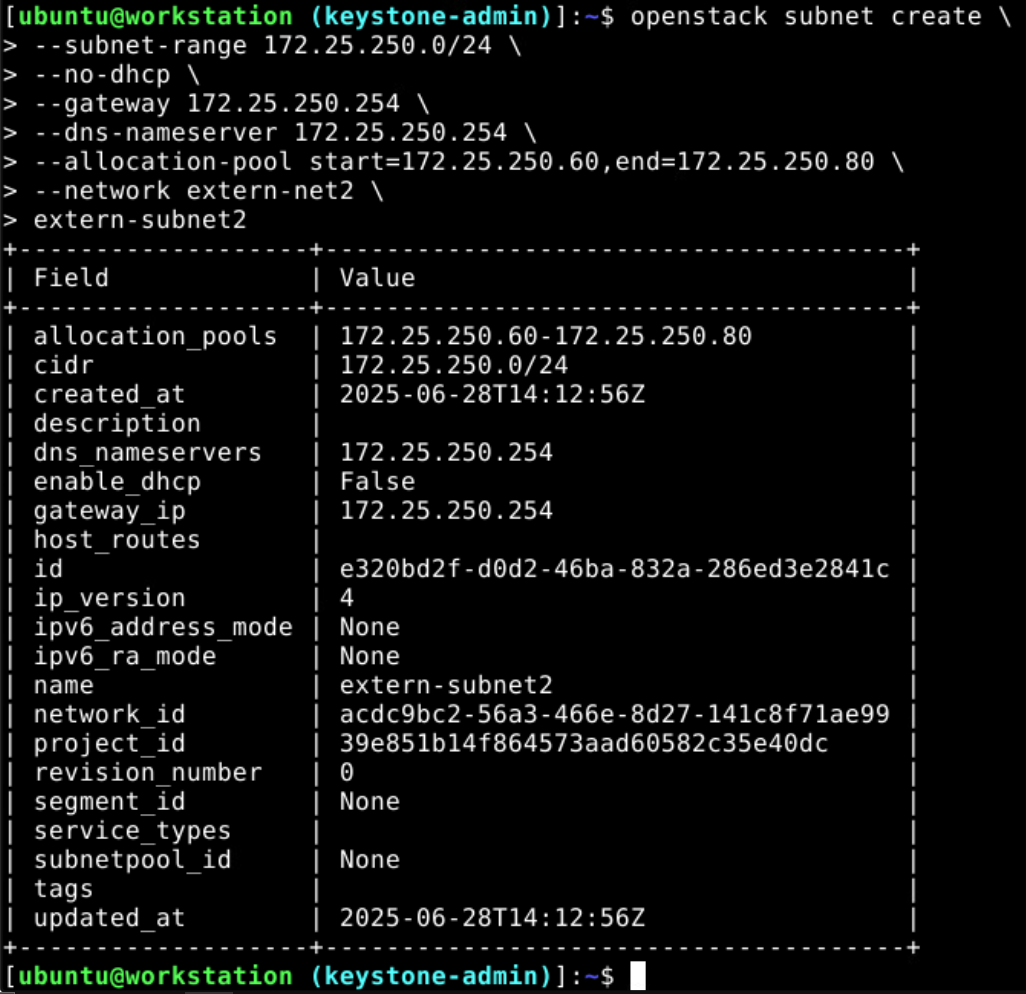
\includegraphics[width=\linewidth]{images/part1/step16.png}
        \end{center}
    \end{labstep}

    \begin{labstep}
        List the networks again to see that \textbf{extern-net2} and \textbf{extern-subnet2} were created successfully.
        \begin{lstlisting}
            [ubuntu@workstation (keystone-admin)]:~$ openstack network list
        \end{lstlisting}

        \begin{center}
            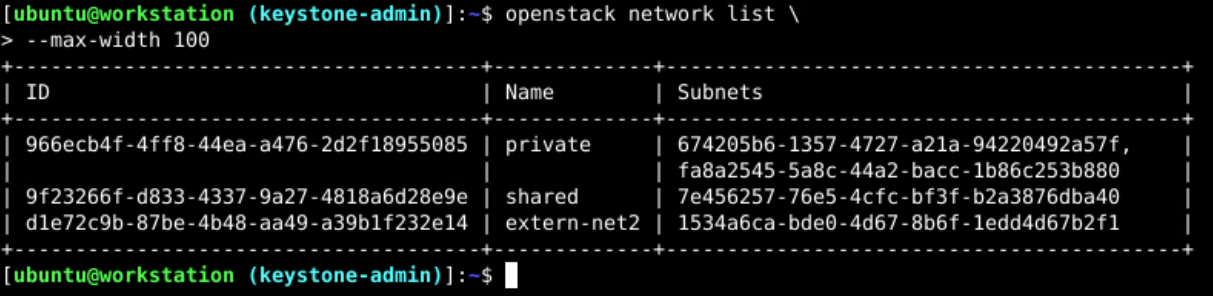
\includegraphics[width=\linewidth]{images/part1/step17.png}
        \end{center}
    \end{labstep}

    \begin{labstep}
        Leave the terminal window open and continue to the next task.
    \end{labstep}

\end{enumerate}

%%%%%%%%%%%
% Section 2
%%%%%%%%%%%
\section{Managing Routers}\label{sec:managing-routers}
In this task, you will create and configure a router with the \textit{Horizon Dashboard} and \textit{OpenStack CLI} and use command line tools to test the connectivity of the router.
The router will serve to connect resources on the external network to other networks both within OpenStack and outside the cloud.

\begin{enumerate}
    \begin{labstep}
        Open the web browser and navigate to \textbf{192.168.1.20}.
        Log into the dashboard as \textbf{admin} with the password \textbf{secret}.
    \end{labstep}

    \begin{labstep}
        Select the \textbf{demo} project and navigate to \textbf{Project $>$ Network $>$ Routers}.
        Click \textbf{Create Router} to create a new router.

        \begin{center}
            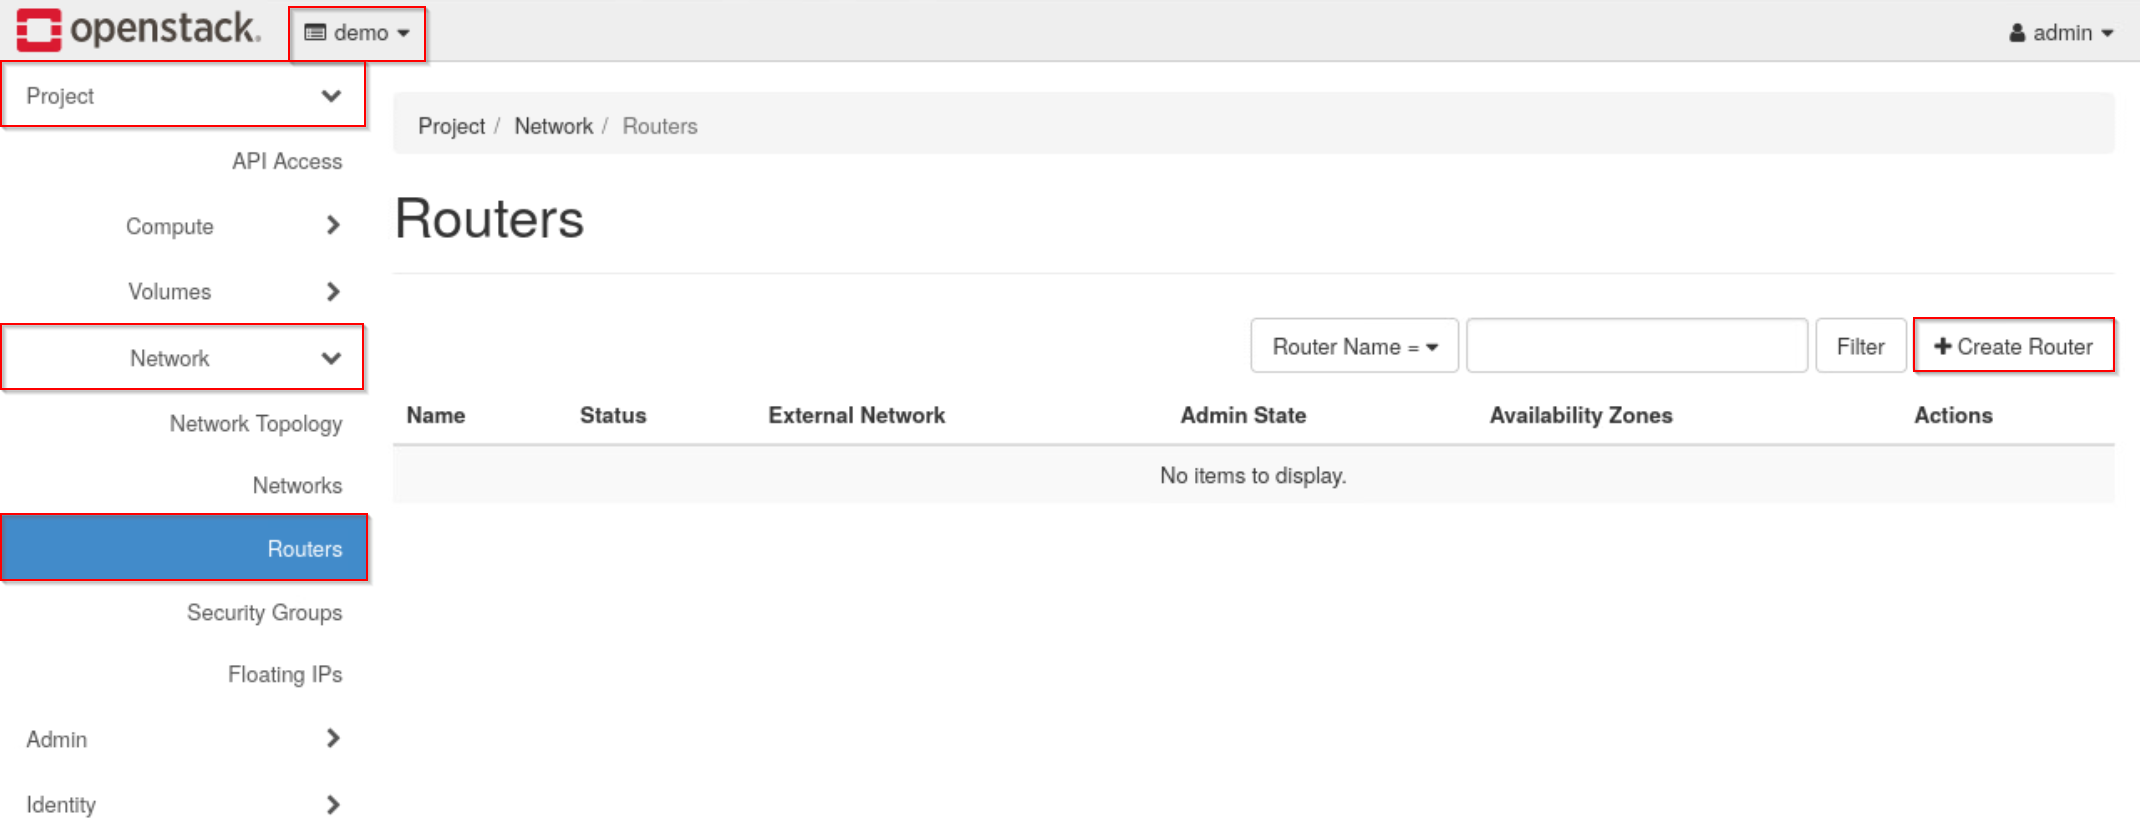
\includegraphics[width=\linewidth]{images/part2/step2.png}
        \end{center}
    \end{labstep}

    \begin{labstep}
        Enter \textbf{router1} in the \textit{Router Name} field and select \textbf{extern-net2} in the \textit{External Network} dropdown.
        Click \textbf{Create Router}.

        \begin{center}
            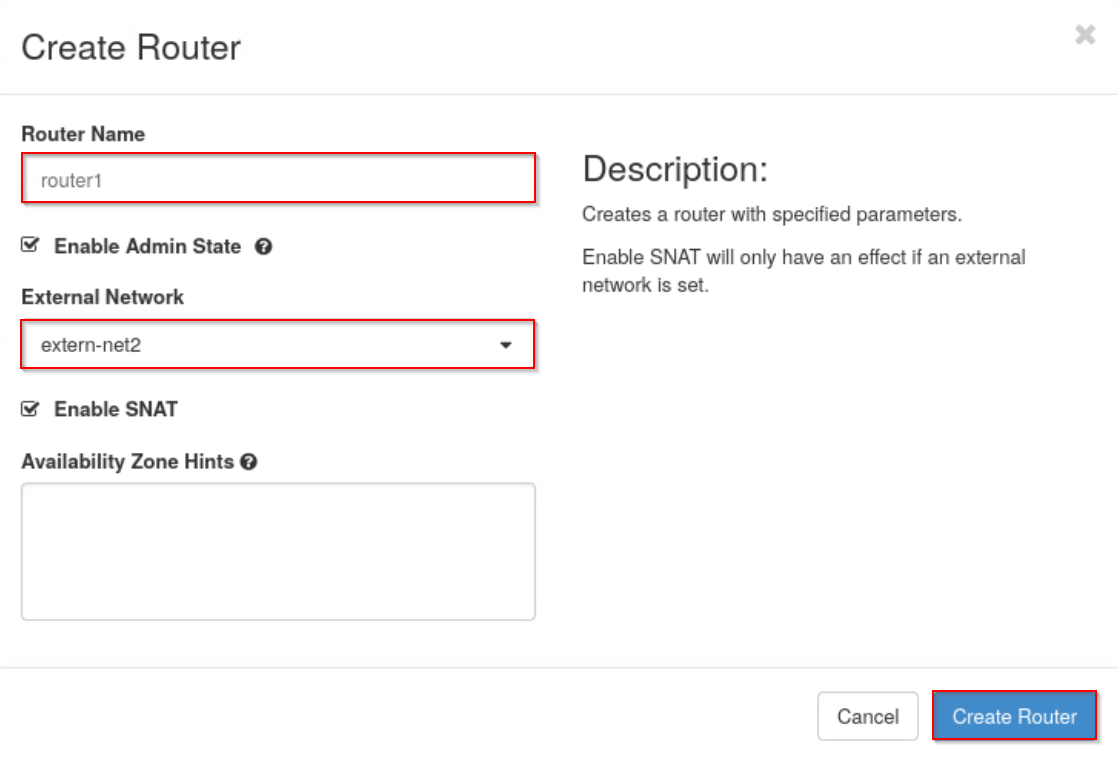
\includegraphics[scale=0.5]{images/part2/step3.png}
        \end{center}
    \end{labstep}

    \begin{labstep}
        Click the router name, \textbf{router1}, to access its details.

        \begin{center}
            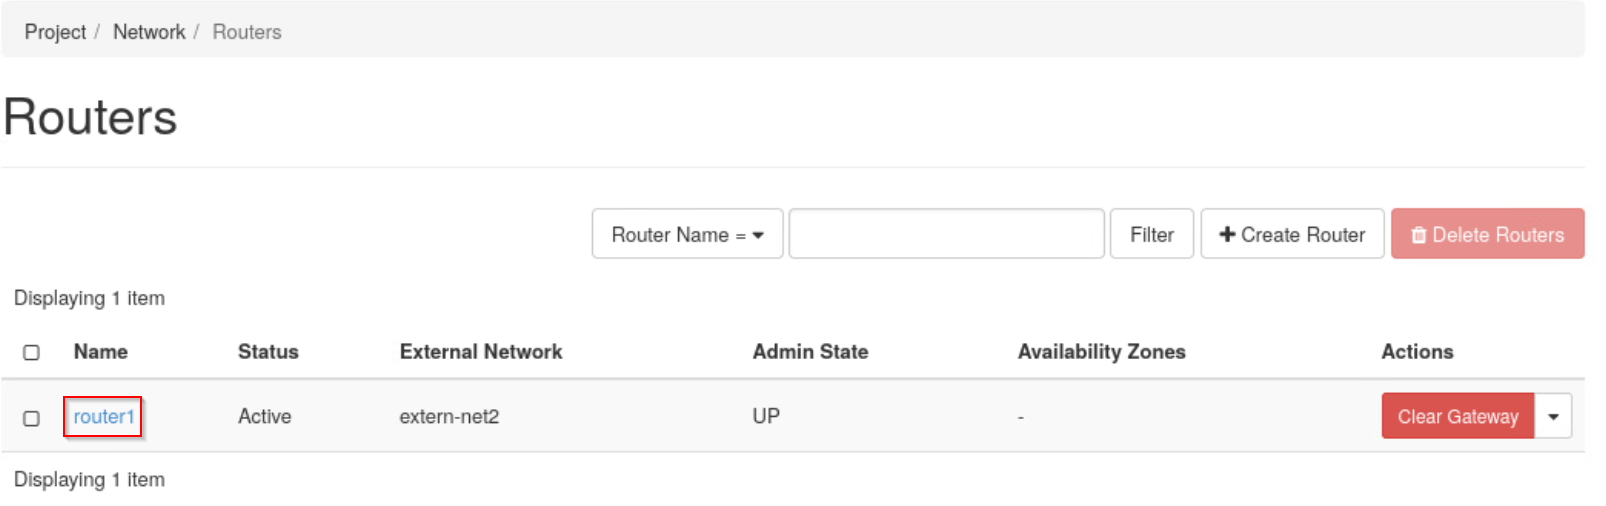
\includegraphics[width=\linewidth]{images/part2/step4.png}
        \end{center}
    \end{labstep}

    \begin{labstep}
        Click the \textbf{Interfaces} tab to manage the interfaces for the router.
        Notice that currently, the router only has an interface connecting it to the \textbf{extern-net2} external network.
        This will connect instances on this network to networks outside the cloud.
        We will add an interface to connect \textbf{extern-net2} to another network within the OpenStack cloud environment.
        Click \textbf{Add Interface} to add a new interface.

        \begin{center}
            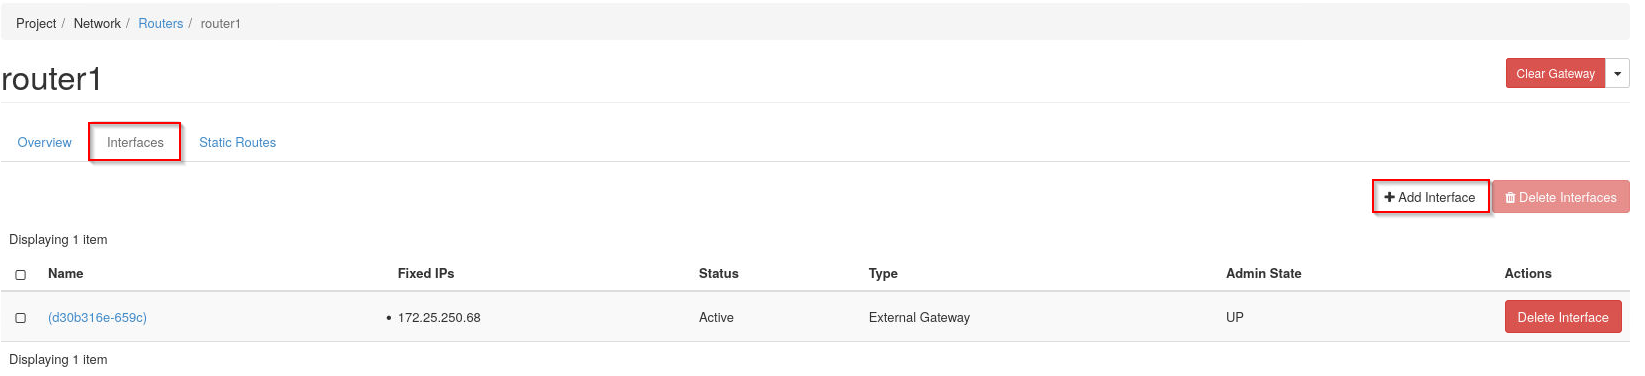
\includegraphics[width=\linewidth]{images/part2/step5.png}
        \end{center}
    \end{labstep}

    \begin{labstep}
        Select \textbf{shared: 192.168.233.0/24 (shared-subnet)} from the \textit{Subnet} dropdown and click \textbf{Submit} to add the interface.
        This will connect the \textbf{extern-net2} network to the \textbf{shared} network.

        \begin{center}
            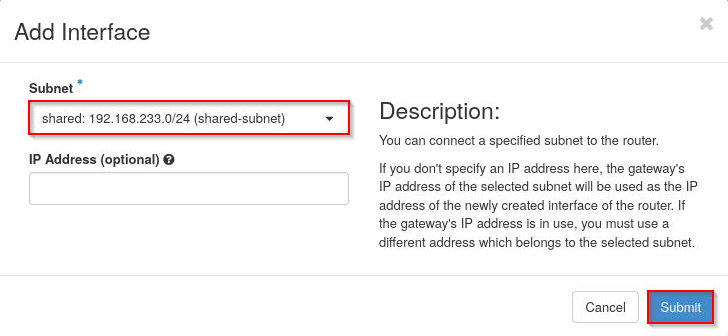
\includegraphics[width=\linewidth]{images/part2/step6.png}
        \end{center}
    \end{labstep}

    \begin{tipbox}
        You can delete an interface by selecting the checkbox next to the interface name, then clicking \textbf{Delete Interfaces}.
        Alternatively, simply click \textbf{Delete Interface} in the same row as the target interface.
    \end{tipbox}

    \begin{labstep}
        Log out of the dashboard and close the web browser.
    \end{labstep}

    \begin{labstep}
        Open a terminal window if one is not already open, and source the \textbf{admin} credentials.
        \begin{lstlisting}
            ubuntu@workstation:~$ source ~/keystonerc-admin
        \end{lstlisting}

        \begin{center}
            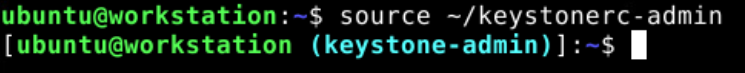
\includegraphics[width=\linewidth]{images/part2/step8.png}
        \end{center}
    \end{labstep}

    \begin{labstep}
        Next, we will recreate this router from the CLI, so we need to delete \textbf{router1}.
        In the Horizon Dashboard, this process is straightforward: deleting a router automatically removes its interfaces.
        However, when using the CLI, the process requires a few extra steps.
        Try deleting \textbf{router1}; you should receive an error.
        \begin{lstlisting}
            [ubuntu@workstation (keystone-admin)]:~$ openstack router delete router1
        \end{lstlisting}

        \begin{center}
            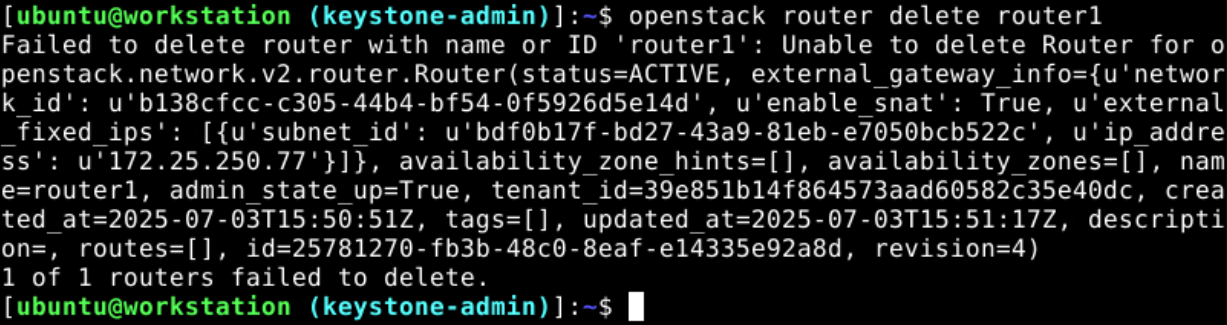
\includegraphics[width=\linewidth]{images/part2/step9.png}
        \end{center}
    \end{labstep}

    \begin{labstep}
        This error occurs because the CLI does not allow a router to be deleted while it is still connected to networks.
        To proceed, we must first disconnect the router by removing any attached subnets.
        In this case, we already know the name of the subnet: \textbf{shared-subnet} on the \textbf{shared} network.
        Later in the lab, you'll learn how to automate this process even when you don't know the names of the router's connected subnets.
        For now, remove the connection to \textbf{shared-subnet}.
        \begin{lstlisting}
            [ubuntu@workstation (keystone-admin)]:~$ openstack router remove subnet \
            > router1 \
            > shared-subnet
        \end{lstlisting}

        \begin{center}
            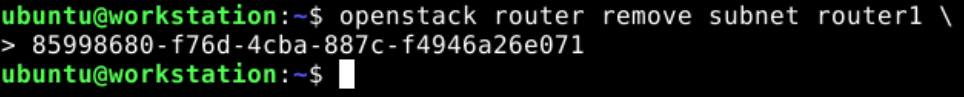
\includegraphics[width=\linewidth]{images/part2/step10.png}
        \end{center}
    \end{labstep}

    \begin{labstep}
        Unset the external gateway of the router.
        \begin{lstlisting}
            [ubuntu@workstation (keystone-admin)]:~$ openstack router unset \
            > --external-gateway router1
        \end{lstlisting}

        \begin{center}
            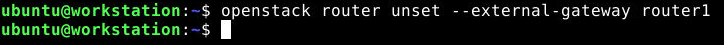
\includegraphics[width=\linewidth]{images/part2/step11.png}
        \end{center}
    \end{labstep}

    \begin{tipbox}
        Since we know that the external gateway goes through \textbf{extern-net2}, we could have also used this command:
        \begin{lstlisting}
            openstack router remove subnet router1 extern-net2
        \end{lstlisting}
    \end{tipbox}

    \begin{labstep}
        Delete the \textbf{router1} router.
        \begin{lstlisting}
            [ubuntu@workstation (keystone-admin)]:~$ openstack router delete router1
        \end{lstlisting}

        \begin{center}
            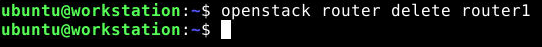
\includegraphics[width=\linewidth]{images/part2/step12.png}
        \end{center}
    \end{labstep}

    \begin{labstep}
        Now, we will replicate the previous router from the CLI.
        Create a router named \textbf{router2}.
        \begin{lstlisting}
            [ubuntu@workstation (keystone-admin)]:~$ openstack router create router2
        \end{lstlisting}

        \begin{center}
            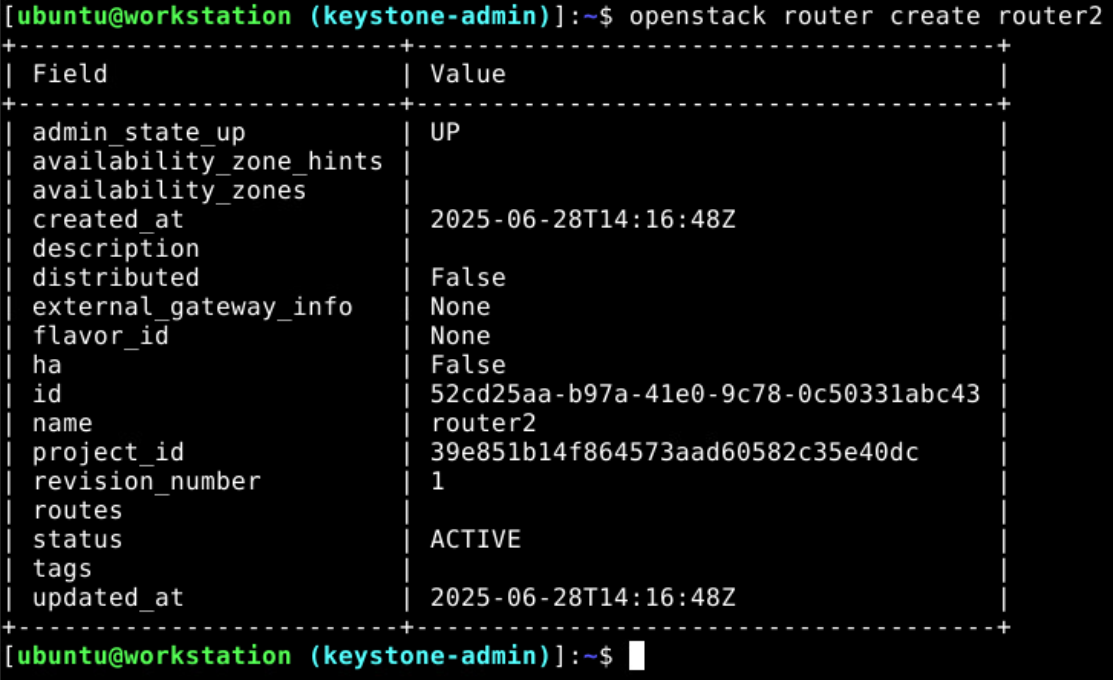
\includegraphics[width=\linewidth]{images/part2/step13.png}
        \end{center}
    \end{labstep}

    \begin{labstep}
        Connect the router to the \textbf{shared-subnet} subnet.
        \begin{lstlisting}
            [ubuntu@workstation (keystone-admin)]:~$ openstack router add subnet \
            > router2 \
            > shared-subnet
        \end{lstlisting}

        \begin{center}
            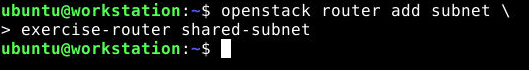
\includegraphics[width=\linewidth]{images/part2/step14.png}
        \end{center}
    \end{labstep}

    \begin{labstep}
        Set the \textbf{extern-net2} network as the gateway for the router.
        \begin{lstlisting}
            [ubuntu@workstation (keystone-admin)]:~$ openstack router set \
            > --external-gateway extern-net2 \
            > router2
        \end{lstlisting}

        \begin{center}
            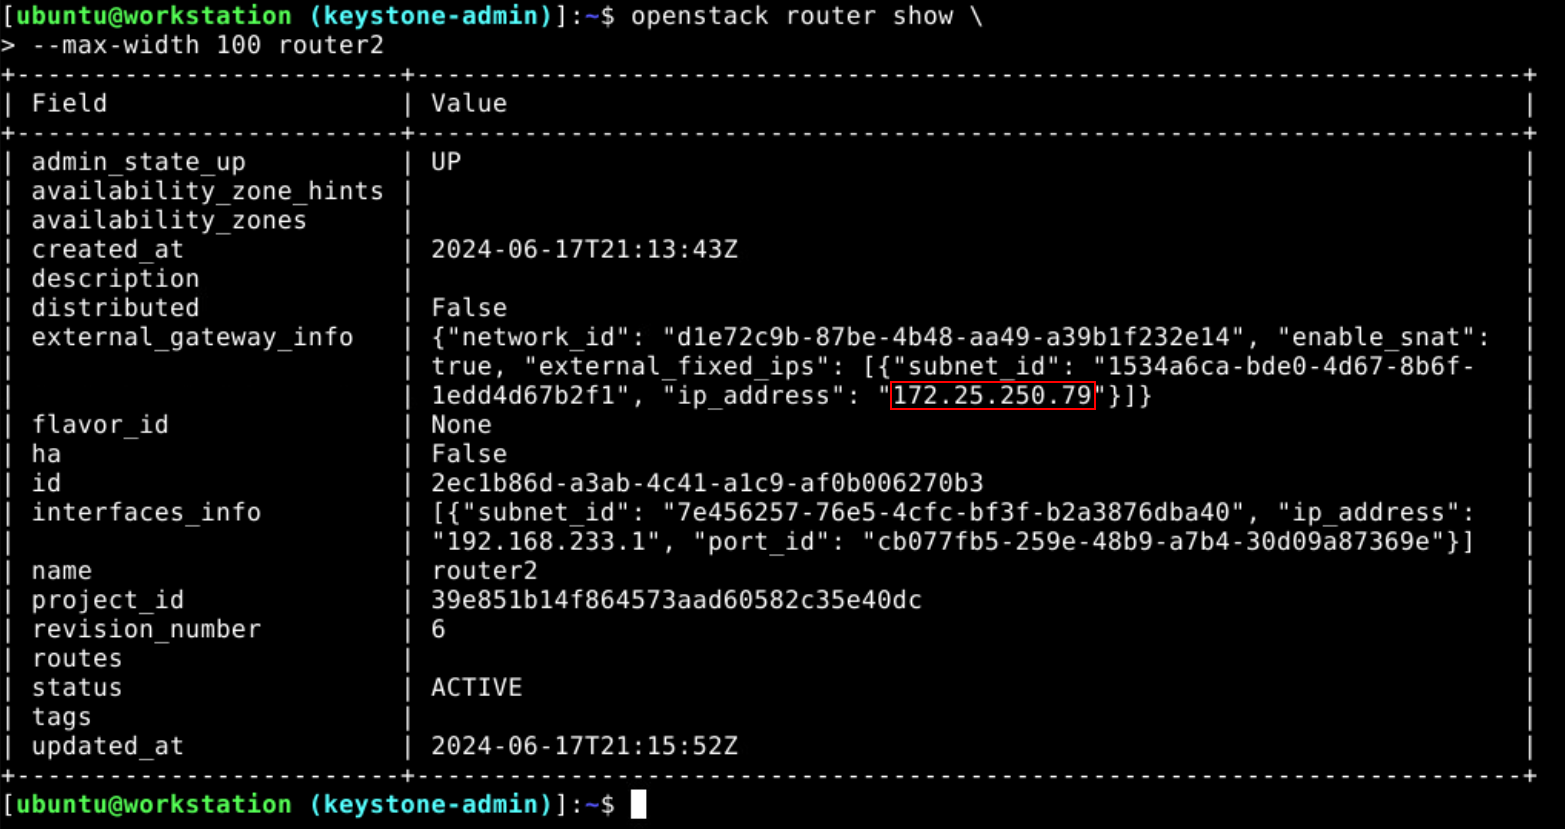
\includegraphics[width=\linewidth]{images/part2/step15.png}
        \end{center}
    \end{labstep}

    \begin{labstep}
        Show the details of the \textbf{router2} router.
        Take note of the IP address listed in the \textit{external\_gateway\_info} row, as you will ping this address in a later step to verify that the router can be reached.
        \begin{lstlisting}
            [ubuntu@workstation (keystone-admin)]:~$ openstack router show router2
        \end{lstlisting}

        \begin{center}
            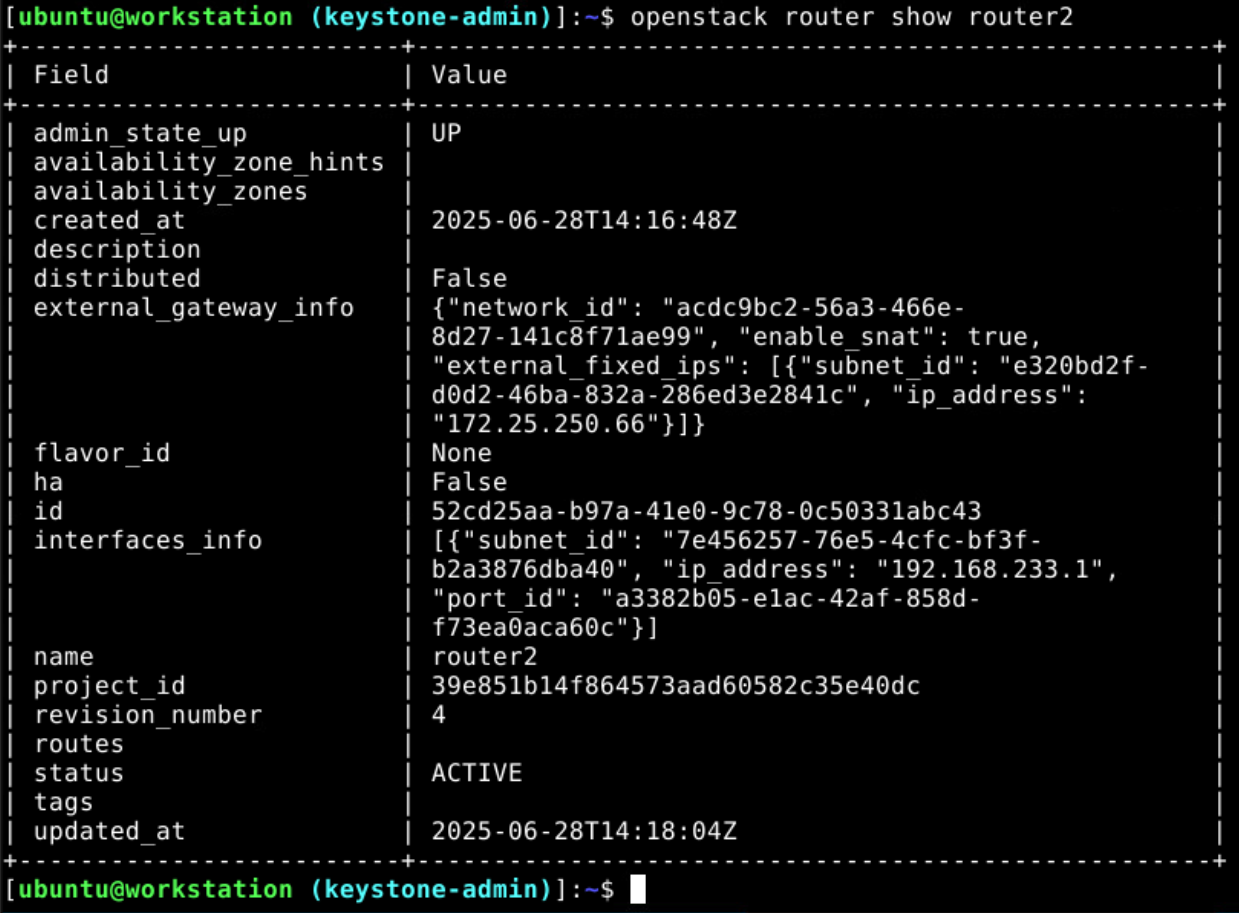
\includegraphics[scale=0.4]{images/part2/step16.png}
        \end{center}
    \end{labstep}

    \begin{labstep}
        In order to test the connectivity of the router, SSH into the \textbf{devstack} virtual machine.
        Log in with the password \textbf{ubuntu}.
        \begin{lstlisting}
            [ubuntu@workstation (keystone-admin)]:~$ ssh 192.168.1.20
        \end{lstlisting}

        \begin{center}
            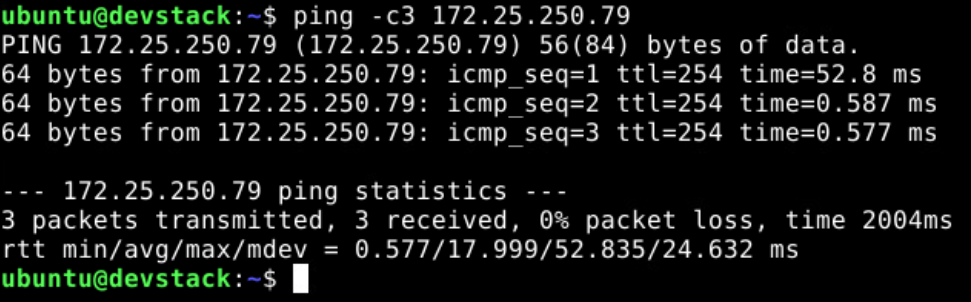
\includegraphics[width=\linewidth]{images/part2/step17.png}
        \end{center}
    \end{labstep}

    \begin{labstep}
        Use the \textbf{ping} command on the IP address found from the \textbf{openstack router show} command to verify that the router can be reached.
        Receiving ping replies verifies the connectivity of the router since the \textbf{devstack} machine is outside the OpenStack cloud environment.
        \begin{lstlisting}
            ubuntu@devstack:~$ ping -c3 172.25.250.66
        \end{lstlisting}

        \begin{center}
            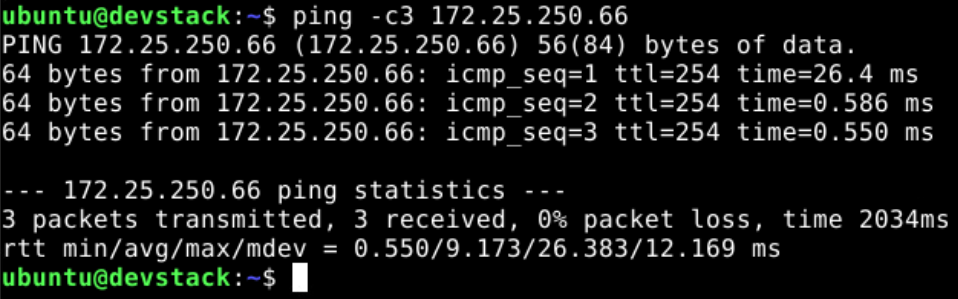
\includegraphics[width=\linewidth]{images/part2/step18.png}
        \end{center}
    \end{labstep}

    \begin{notebox}
        The actual IP address may differ from this example.
    \end{notebox}
    \begin{notebox}
        You should receive three successful ping replies.
    \end{notebox}

    \begin{labstep}
        Exit the SSH session.
        \begin{lstlisting}
            ubuntu@devstack:~$ exit
        \end{lstlisting}

        \begin{center}
            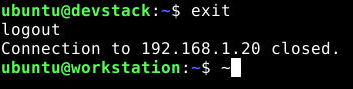
\includegraphics[width=\linewidth]{images/part2/step19.png}
        \end{center}
    \end{labstep}

    \begin{labstep}
        Leave the terminal window open and continue to the next task.
    \end{labstep}

\end{enumerate}

%%%%%%%%%%%
% Section 3
%%%%%%%%%%%
\section{Managing Floating IP Addresses}\label{sec:managing-floating-ip-addresses}
In this task, you will create a floating IP address and allocate it to an instance with the \textit{Horizon Dashboard} and the \textit{OpenStack Unified CLI}.
Instances are assigned a private, fixed IP address at creation to communicate with other instances.
However, they can also be assigned a floating IP address, which can be exchanged at any time and is used for communication outside the OpenStack cloud environment.

\begin{enumerate}
    \begin{labstep}
        If a terminal window is not already open, open one and source the admin credentials from the \textbf{\texttildemid/keystonerc-admin} file.
        \begin{lstlisting}
            ubuntu@workstation:~$ source ~/keystonerc-admin
        \end{lstlisting}

        \begin{center}
            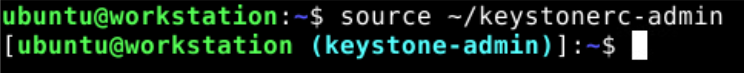
\includegraphics[width=\linewidth]{images/part3/step1.png}
        \end{center}
    \end{labstep}

    \begin{labstep}
        Create a new instance named \textbf{instance1}.
        Use the \textbf{ubuntu} image, \textbf{m1.small} flavor, and \textbf{shared} network.
        \begin{lstlisting}
            [ubuntu@workstation (keystone-admin)]:~$ openstack server create \
            > --image ubuntu \
            > --flavor m1.small \
            > --network shared \
            > instance1
        \end{lstlisting}

        \begin{center}
            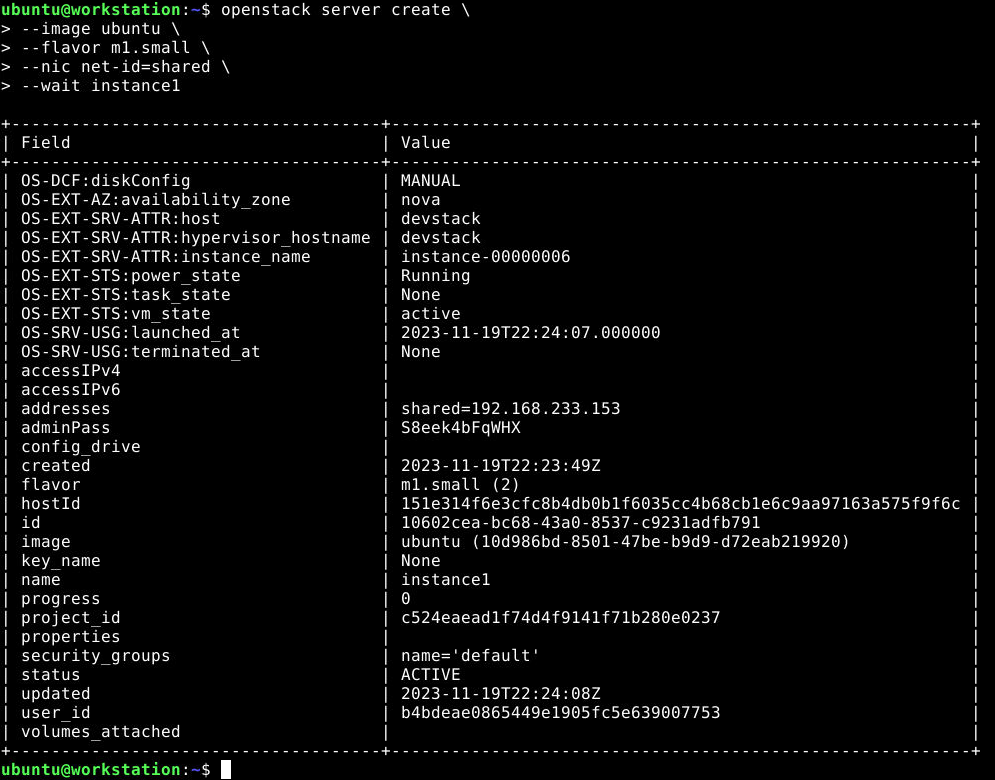
\includegraphics[width=\linewidth]{images/part3/step2.png}
        \end{center}
    \end{labstep}

    \begin{labstep}
        Leave the terminal window open and open the web browser.
        Navigate to \textbf{192.168.1.20}.
        Log into the \textit{Horizon Dashboard} as the \textbf{admin} user with the password \textbf{secret}.
    \end{labstep}

    \begin{labstep}
        Select the \textbf{demo} project.
        Navigate to \textbf{Project $>$ Network $>$ Floating IPs}.
        Click \textbf{Allocate IP to Project}.

        \begin{center}
            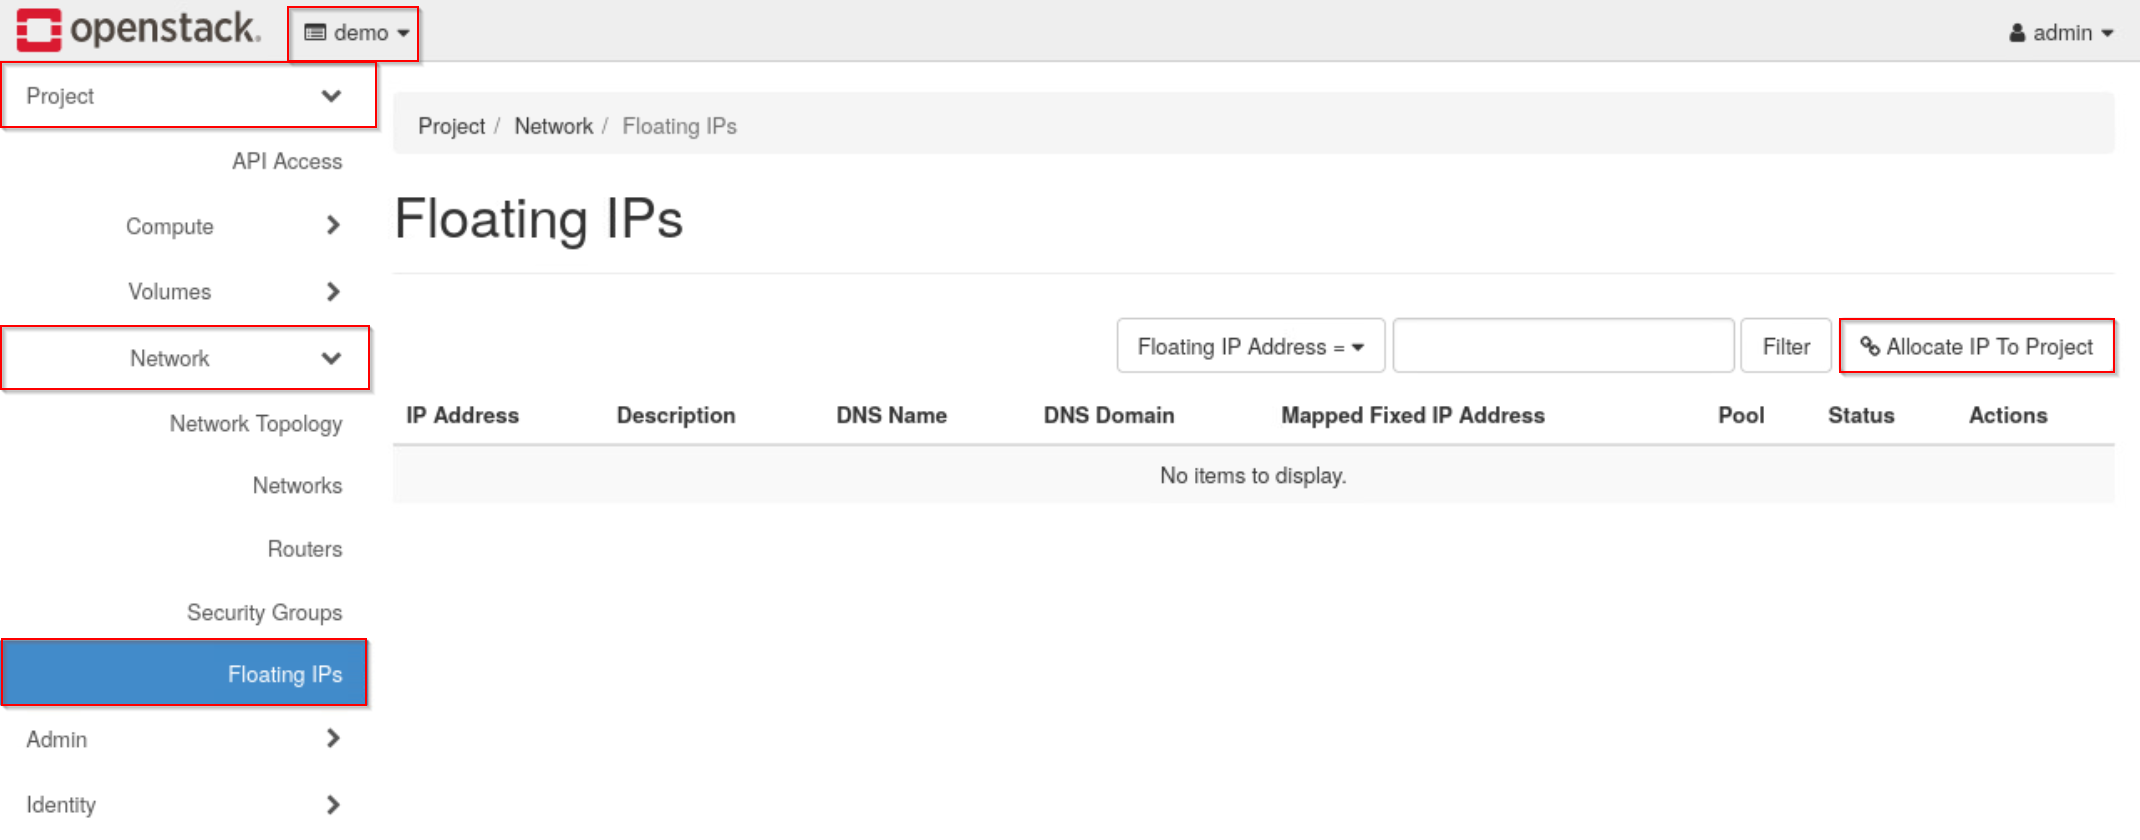
\includegraphics[width=\linewidth]{images/part3/step4.png}
        \end{center}
    \end{labstep}

    \begin{labstep}
        Ensure \textbf{extern-net2} is set as the \textit{Pool}.
        Click \textbf{Allocate IP}.

        \begin{center}
            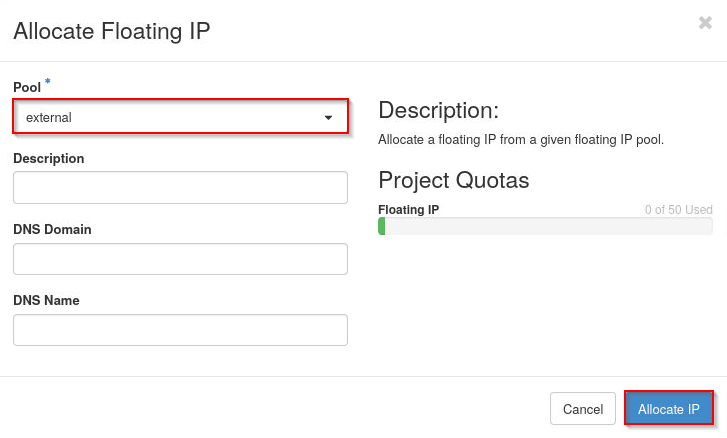
\includegraphics[width=\linewidth]{images/part3/step5.png}
        \end{center}
    \end{labstep}

    \begin{tipbox}
        A floating IP address can be deleted, or released, in multiple ways.
        One way is to select the checkbox next to the floating IP address, and click \textbf{Release Floating IPs}.
        Another way is to open the dropdown next to the \textbf{Associate} button in the same row as the floating IP address, then click \textbf{Release Floating IP}.
    \end{tipbox}

    \begin{labstep}
        Click \textbf{Associate} in the row of the floating IP address.

        \begin{center}
            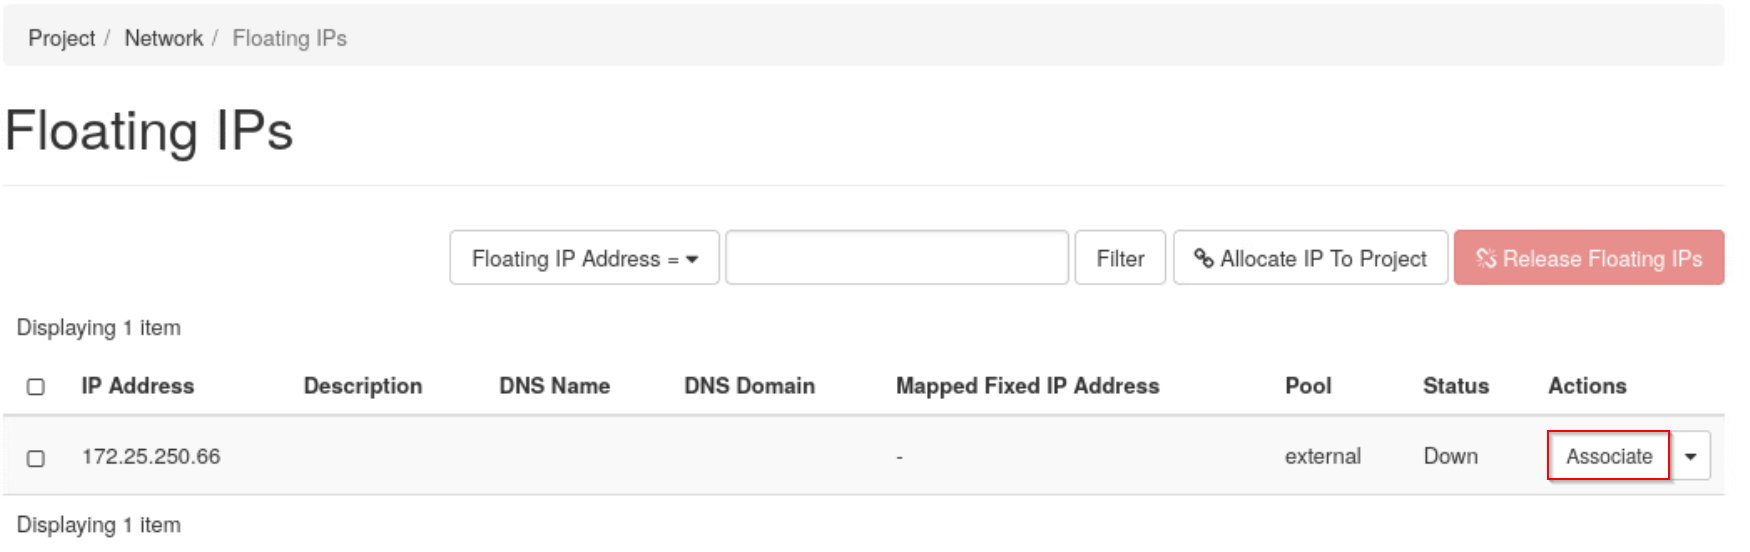
\includegraphics[width=\linewidth]{images/part3/step6.png}
        \end{center}
    \end{labstep}

    \begin{notebox}
        The actual value of the floating IP address may differ.
    \end{notebox}

    \begin{labstep}\label{it:floating-ip}
        In the \textit{Port to be associated} dropdown, select \textbf{instance1: 192.168.233.XYZ}.
        Click \textbf{Associate}.

        \begin{center}
            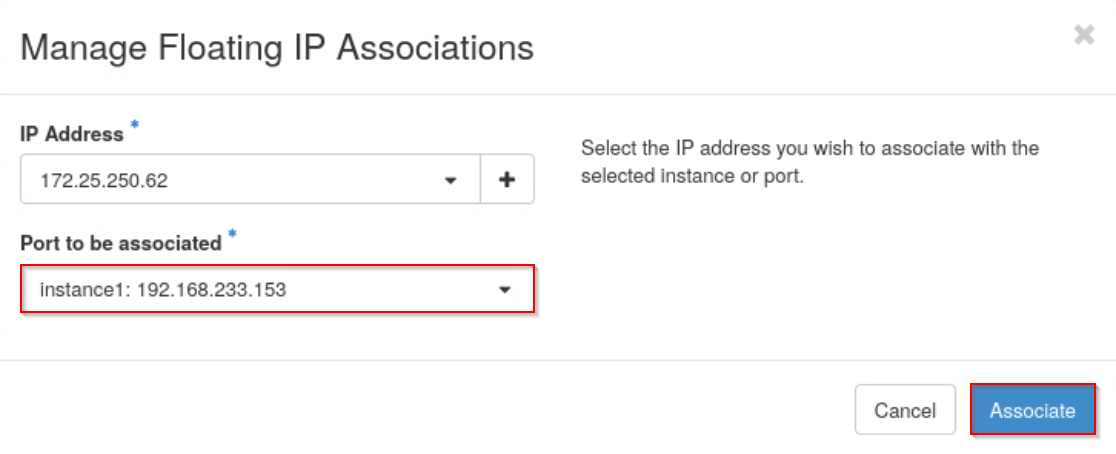
\includegraphics[width=\linewidth]{images/part3/step7.png}
        \end{center}
    \end{labstep}

    \begin{notebox}
        The actual value of the instance's IP address may differ.
    \end{notebox}

    \begin{labstep}
        The \textbf{instance1} instance is now connected to the \textbf{extern-net2} network through its floating IP address.
        At this point, it might seem like the instance should be accessible from a network outside the OpenStack environment.
        This is a reasonable assumption because the router is accessible, the instance is connected to it, and a floating IP address has been assigned.
        However, OpenStack applies a ``Deny by Default'' security model, which means inbound (ingress) traffic to the instance is blocked unless explicitly allowed by security group rules.
        We'll configure those rules in the next lab.
        For now, let's verify that \textbf{instance1} is \textit{not} reachable.
        Open a terminal window (if you haven't already), and SSH into the \textbf{devstack} virtual machine.
        Log in with the password \textbf{ubuntu}.
        \begin{lstlisting}
            [ubuntu@workstation (keystone-admin)]:~$ ssh 192.168.1.20
        \end{lstlisting}

        \begin{center}
            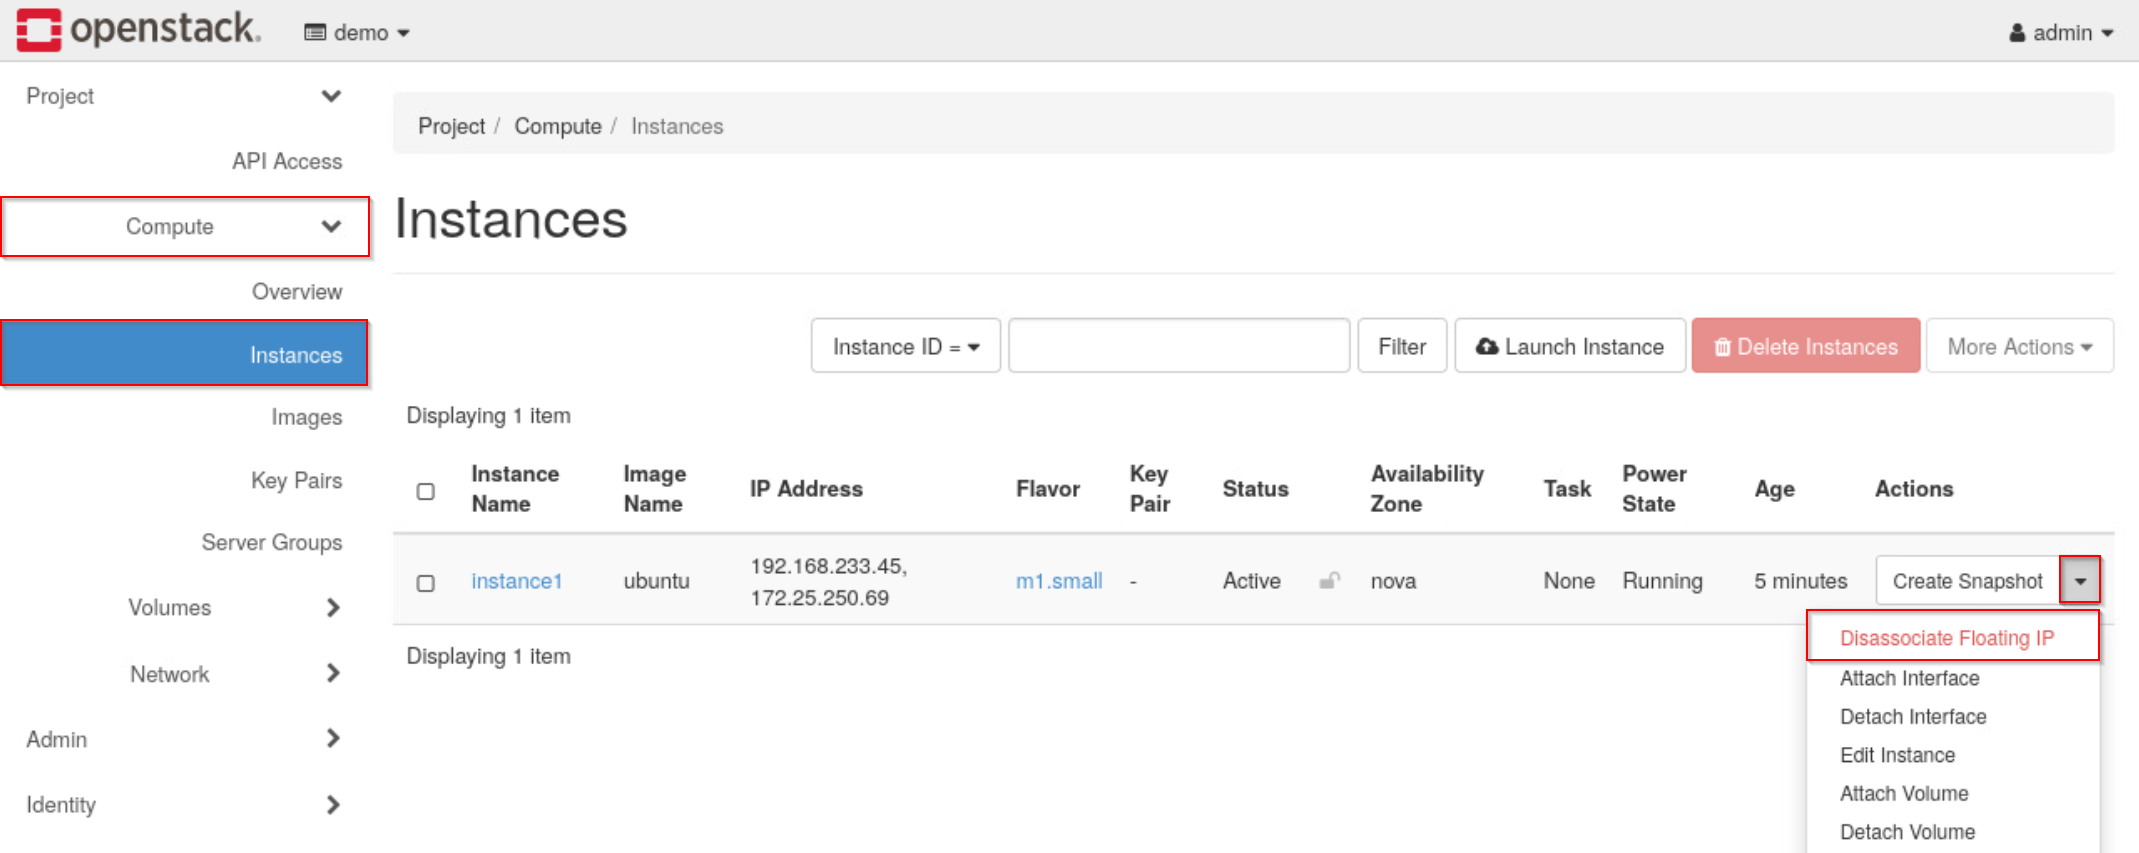
\includegraphics[width=\linewidth]{images/part3/step8.png}
        \end{center}
    \end{labstep}

    \begin{labstep}
        Use the \textbf{ping} command on the floating IP address that was associated with \textbf{instance1} in step~\ref{it:floating-ip}.
        \begin{lstlisting}
            ubuntu@devstack:~$ ping -c3 172.25.250.62
        \end{lstlisting}

        \begin{center}
            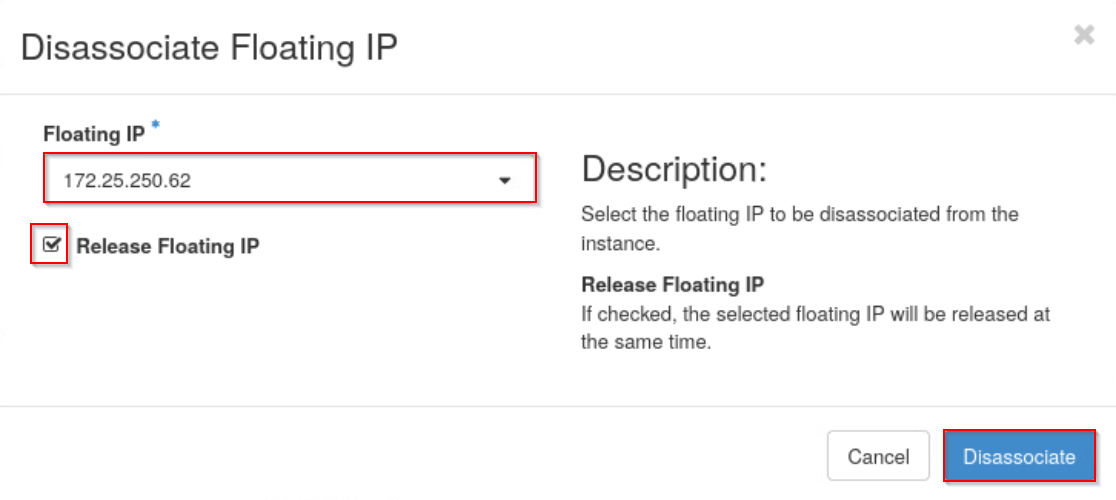
\includegraphics[width=\linewidth]{images/part3/step9.png}
        \end{center}
    \end{labstep}

    \begin{notebox}
        You should not receive any ping replies.
        Instead, the output of the command should inform you that there was 100\% packet loss.
        This confirms that although the network is configured correctly, the instance is still protected by default security group rules that block incoming traffic.
        We will set up these security rules in the next lab and see that the instance can be successfully reached after that.
    \end{notebox}

    \begin{labstep}
        Exit the SSH session.
        \begin{lstlisting}
            ubuntu@devstack:~$ exit
        \end{lstlisting}

        \begin{center}
            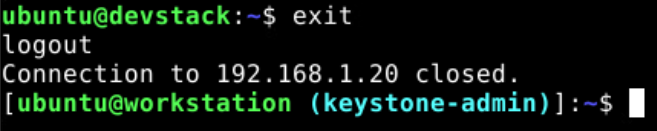
\includegraphics[width=\linewidth]{images/part3/step10.png}
        \end{center}
    \end{labstep}

    \begin{labstep}
        We are now finished with this floating IP address.
        Return to the web browser.
        To remove a floating IP address, first navigate to \textbf{Compute $>$ Instances}.
        Click the arrow next to the \textbf{Create Snapshot} in the same as \textbf{instance1}.
        Select \textbf{Disassociate Floating IP} to detach the floating IP from the instance.

        \begin{center}
            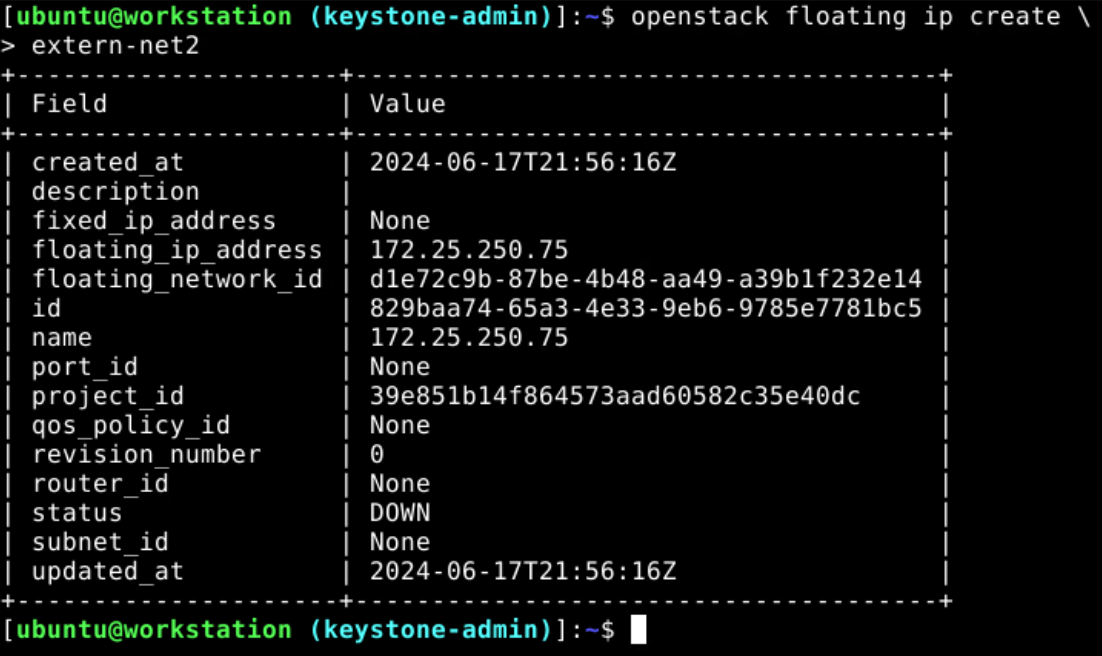
\includegraphics[width=\linewidth]{images/part3/step11.png}
        \end{center}
    \end{labstep}

    \begin{labstep}
        Check the \textit{Release Floating IP} box and click \textbf{Disassociate}.

        \begin{center}
            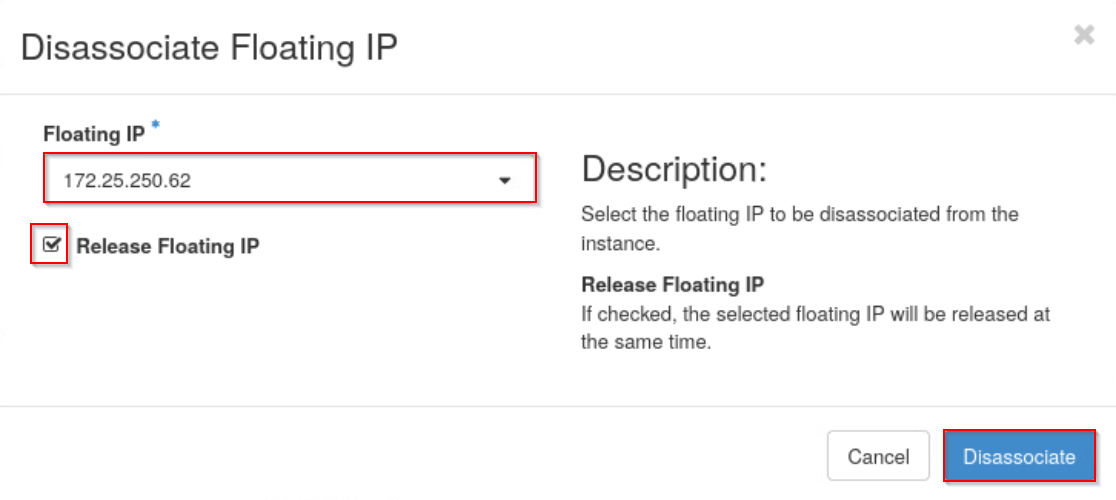
\includegraphics[width=\linewidth]{images/part3/step12.png}
        \end{center}
    \end{labstep}

    \begin{tipbox}
        A floating IP address can also be disassociated from the \textbf{Project $>$ Network $>$ Floating IPs} page.
        When a floating IP address has been associated with an instance, the button in the row of the floating IP address that used to read \textbf{Associate} will turn red and read \textbf{Disassociate}.
        Clicking this button will disassociate the floating IP address from its instance.
    \end{tipbox}

    \begin{labstep}
        Log out of the \textit{Horizon Dashboard} and close the web browser.
    \end{labstep}

    \begin{labstep}
        From the terminal, allocate a floating IP address in the \textbf{extern-net2} network.
        \begin{lstlisting}
            [ubuntu@workstation (keystone-admin)]:~$ openstack floating ip create \
            > extern-net2
        \end{lstlisting}

        \begin{center}
            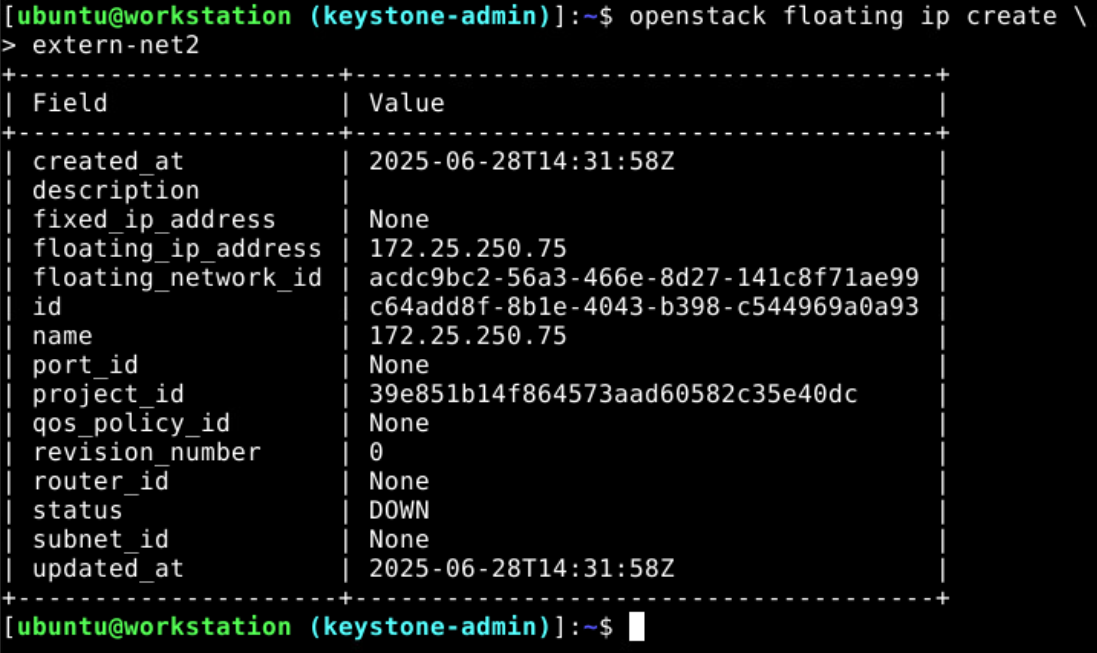
\includegraphics[width=\linewidth]{images/part3/step14.png}
        \end{center}
    \end{labstep}

    \begin{labstep}
        Notice that the previous command generated a random floating IP address within the allocation pool.
        You can use the \textbf{--floating-ip-address} argument to allocate a specific IP address.
        However, make sure to list the available addresses before attempting to allocate it.
        If that particular floating IP address already exists, the command will throw an HTTP exception.
        \begin{lstlisting}
            [ubuntu@workstation (keystone-admin)]:~$ openstack floating ip list
        \end{lstlisting}

        \begin{center}
            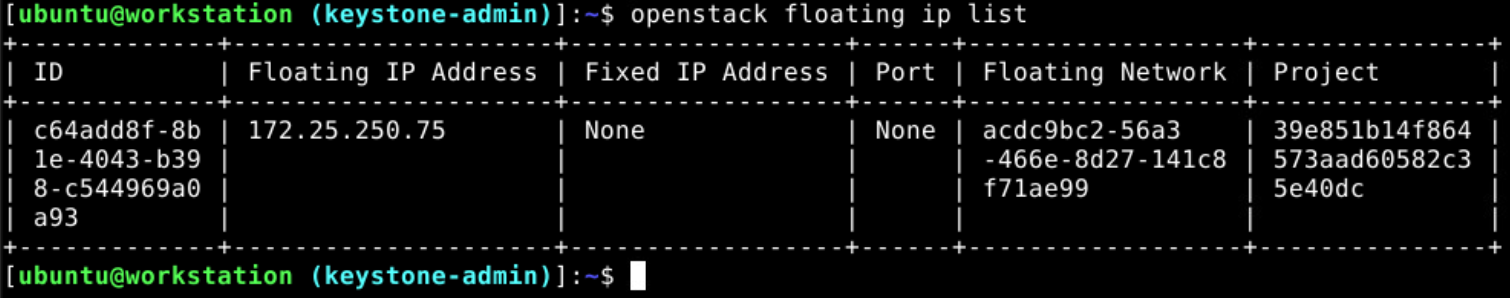
\includegraphics[width=\linewidth]{images/part3/step15.png}
        \end{center}
    \end{labstep}

    \begin{tipbox}
        This command does not properly fit the width of its output until you expand or maximize your terminal window.
        Alternatively, appending arguments such as \textbf{-c ``Floating IP Address'' -c ``Fixed IP Address''} to output only the columns you need can make the output easier to read. % chktex 18
    \end{tipbox}

    \begin{labstep}
        Create the floating IP address \textbf{172.25.250.80}.
        \begin{lstlisting}
            [ubuntu@workstation (keystone-admin)]:~$ openstack floating ip create \
            > --floating-ip-address 172.25.250.80 \
            > extern-net2
        \end{lstlisting}

        \begin{center}
            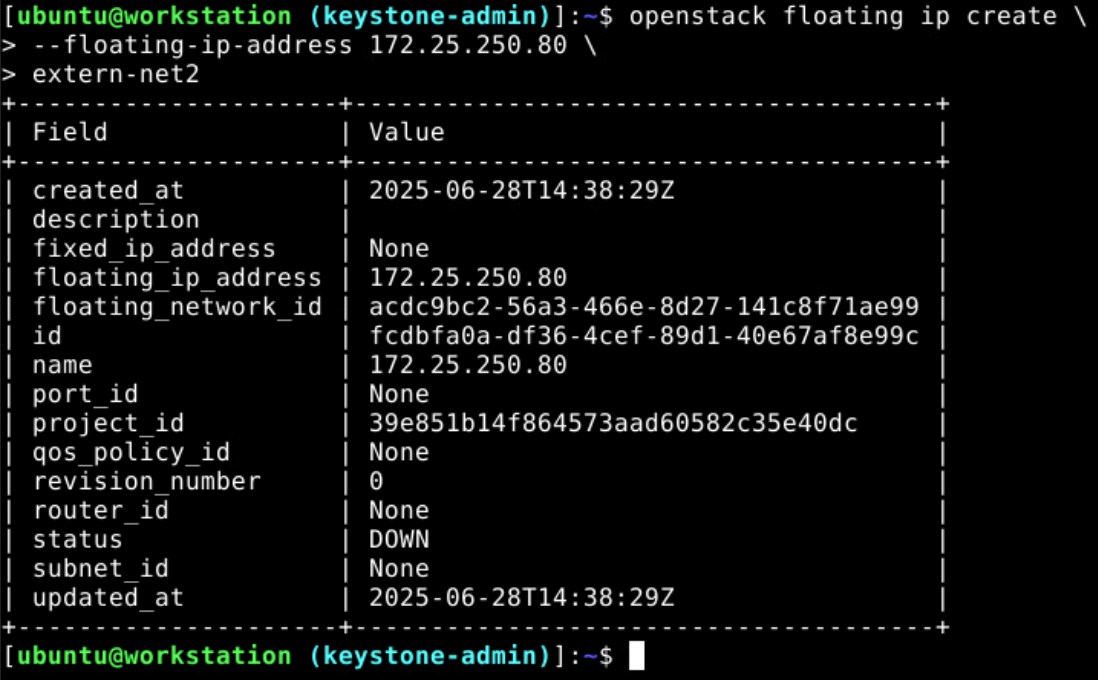
\includegraphics[scale=0.5]{images/part3/step16.png}
        \end{center}
    \end{labstep}

    \begin{labstep}
        Try creating the same floating IP address again.
        This time, it should raise an HTTP exception.
        \begin{lstlisting}
            [ubuntu@workstation (keystone-admin)]:~$ openstack floating ip create \
            > --floating-ip-address 172.25.250.80 \
            > extern-net2
        \end{lstlisting}

        \begin{center}
            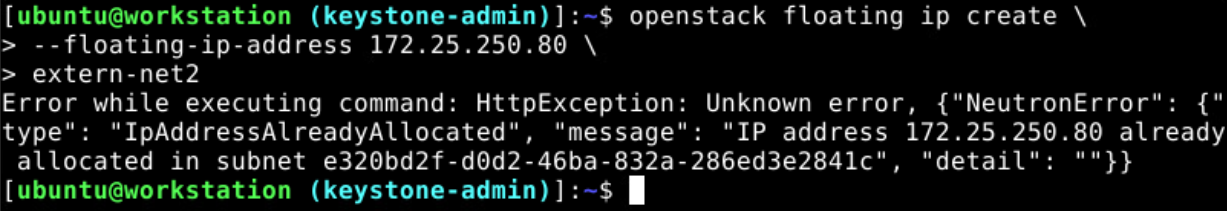
\includegraphics[width=\linewidth]{images/part3/step17.png}
        \end{center}
    \end{labstep}

    \begin{labstep}
        Associate this floating IP address with \textbf{instance1}.
        \begin{lstlisting}
            [ubuntu@workstation (keystone-admin)]:~$ openstack server add floating ip \
            > instance1 \
            > 172.25.250.80
        \end{lstlisting}

        \begin{center}
            \includegraphics[width=\linewidth]{images/part3/step18.png}
        \end{center}
    \end{labstep}

    \begin{labstep}
        List the details of \textbf{instance1} to verify that the floating IP address was attached.
        The \textbf{Networks} column should list both the internal and floating IP address of the instance.
        \begin{lstlisting}
            [ubuntu@workstation (keystone-admin)]:~$ openstack server list
        \end{lstlisting}

        \begin{center}
            \includegraphics[width=\linewidth]{images/part3/step19.png}
        \end{center}
    \end{labstep}

    \begin{labstep}
        We are now finished with this floating IP address, so it can be removed from the instance and deleted.
        Remove the floating IP address from \textbf{instance1}.
        \begin{lstlisting}
            [ubuntu@workstation (keystone-admin)]:~$ openstack floating ip remove \
            > instance1 \
            > 172.25.250.80
        \end{lstlisting}

        \begin{center}
            \includegraphics[width=\linewidth]{images/part3/step20.png}
        \end{center}
    \end{labstep}

    \begin{tipbox}
        This command is equivalent to clicking \textbf{Disassociate} in the Horizon Dashboard, and it is useful when you want to reuse the IP address for something else.
        However, a floating IP address can be deleted without first removing it from the instance.
    \end{tipbox}

    \begin{labstep}
        When a floating IP address is removed from an instance, it still exists and is available to add to another instance.
        List the available floating IP addresses to confirm this.
        \begin{lstlisting}
            [ubuntu@workstation (keystone-admin)]:~$ openstack floating ip list
        \end{lstlisting}

        \begin{center}
            \includegraphics[width=\linewidth]{images/part3/step21.png}
        \end{center}
    \end{labstep}

    \begin{labstep}
        Delete the floating IP address \textbf{172.25.250.80}.
        \begin{lstlisting}
            [ubuntu@workstation (keystone-admin)]:~$ openstack floating ip delete \
            > 172.25.250.80
        \end{lstlisting}

        \begin{center}
            \includegraphics[width=\linewidth]{images/part3/step22.png}
        \end{center}
    \end{labstep}

    \begin{labstep}
        One floating IP address we originally created at the beginning of this section still exists.
        Associate this address with \textbf{instance1}.
        \begin{lstlisting}
            [ubuntu@workstation (keystone-admin)]:~$ openstack server add floating ip \
            > instance1 \
            > 172.25.250.75
        \end{lstlisting}

        \begin{center}
            \includegraphics[width=\linewidth]{images/part3/step23.png}
        \end{center}
    \end{labstep}

    \begin{notebox}
        The actual floating IP may differ.
    \end{notebox}

    \begin{labstep}
        Verify that the floating IP address was added to the instance.
        \begin{lstlisting}
            [ubuntu@workstation (keystone-admin)]:~$ openstack server list
        \end{lstlisting}

        \begin{center}
            \includegraphics[width=\linewidth]{images/part3/step24.png}
        \end{center}
    \end{labstep}

    \begin{labstep}
        We will not need this instance anymore, so delete it.
        This will also disassociate the floating IP address, but it will still be available.
        \begin{lstlisting}
            [ubuntu@workstation (keystone-admin)]:~$ openstack server delete instance1
        \end{lstlisting}

        \begin{center}
            \includegraphics[width=\linewidth]{images/part3/step25.png}
        \end{center}
    \end{labstep}

    \begin{labstep}
        Verify that the instance was deleted.
        \begin{lstlisting}
            [ubuntu@workstation (keystone-admin)]:~$ openstack server list
        \end{lstlisting}

        \begin{center}
            \includegraphics[width=\linewidth]{images/part3/step26.png}
        \end{center}
    \end{labstep}

    \begin{labstep}
        Verify that the floating IP address still exists and that it has no fixed IP address (it is not associated with an instance).
        \begin{lstlisting}
            [ubuntu@workstation (keystone-admin)]:~$ openstack floating ip list
        \end{lstlisting}

        \begin{center}
            \includegraphics[width=\linewidth]{images/part3/step27.png}
        \end{center}
    \end{labstep}

    \begin{labstep}
        Leave the terminal window open and continue to the next task.
    \end{labstep}

\end{enumerate}

%%%%%%%%%%%
% Section 4
%%%%%%%%%%%
\section{Deleting Routers and External Networks from the CLI}\label{sec:deleting_routers_and_external_networks_from_the_cli}
Earlier in the lab, you deleted a router by manually removing its connected subnets, since you already knew their names.
While that approach works in simple cases, it doesn't scale well to routers with many interfaces or when subnet names aren't known in advance.
In this task, you will use the \textit{OpenStack Unified CLI} to clean up the environment by deleting the router and external network you previously created.
This time, you'll use a more flexible and automated approach that works even when subnet names are unknown.
You will also learn a few useful tricks for working with commands that require resource IDs as arguments, which will be helpful when writing cleanup scripts or handling more complex environments.

\begin{enumerate}
    \begin{labstep}
        If a terminal window is not already open, open one and source the \textbf{admin} credentials from the
        \textbf{\texttildemid/keystonerc-admin} file.
        \begin{lstlisting}
            ubuntu@workstation:~$ source ~/keystonerc-admin
        \end{lstlisting}

        \begin{center}
            \includegraphics[width=\linewidth]{images/part4/step1.png}
        \end{center}
    \end{labstep}

    \begin{labstep}
        When working from the Horizon Dashboard, a network cannot be deleted if it is connected to a router.
        Although the command line allows them to be deleted in either order, we will still delete the router first.
        Begin by viewing the details of \textbf{router2}.
        \begin{lstlisting}
            [ubuntu@workstation (keystone-admin)]:~$ openstack router show router2
        \end{lstlisting}

        \begin{center}
            \includegraphics[scale=0.45]{images/part4/step2.png}
        \end{center}
    \end{labstep}

    \begin{labstep}
        From the CLI, a router's subnets and interfaces, including its external gateway, must first be cleared before deleting the router.
        Unset the external gateway of \textbf{router2}.
        \begin{lstlisting}
            [ubuntu@workstation (keystone-admin)]:~$ openstack router unset \
            > --external-gateway \
            > router2
        \end{lstlisting}

        \begin{center}
            \includegraphics[width=\linewidth]{images/part4/step3.png}
        \end{center}
    \end{labstep}

    \begin{labstep}
        Next, each of the router's interfaces must be deleted.
        This time, we will specify the interfaces by their IDs.
        To avoid copying and pasting the ID values, we will store them in a variable and delete them at the same time.
        First, list the router's interface IDs.
        \begin{lstlisting}
            [ubuntu@workstation (keystone-admin)]:~$ openstack port list \
            > -c ID \
            > -f value \
            > --router router2
        \end{lstlisting}

        \begin{center}
            \includegraphics[width=\linewidth]{images/part4/step4.png}
        \end{center}
    \end{labstep}

    \begin{notebox}
        The \textbf{-f value} argument specifies that rather than outputting the result in a table format, we want just the value.
        There are a few other output options, such as \textbf{-f json}, but we will not need any other options in these labs.
    \end{notebox}

    \begin{labstep}
        Now, assign the output of the previous step to a variable called \textbf{ports}.
        \begin{lstlisting}
            [ubuntu@workstation (keystone-admin)]:~$ ports=$(!!)
        \end{lstlisting}

        \begin{center}
            \includegraphics[width=\linewidth]{images/part4/step5.png}
        \end{center}
    \end{labstep}

    \begin{tipbox}
        Make sure there are no spaces around the equal sign when assigning a value to a variable.
    \end{tipbox}
    \begin{notebox}
        The \textbf{\$(...)} syntax captures the output of a command, and \textbf{!!} re-executes the immediately preceding command. % chktex 11
        In this case, we could have also used
        \begin{lstlisting}
            ports=$(openstack router port list --router router2 -c ID -f value)
        \end{lstlisting}
        However, this consumes the output of the command and does not print it unless you use the \textbf{echo} command as well.
    \end{notebox}

    \begin{labstep}
        Print the value of the \textbf{ports} variable to make sure it is storing the ID values.
        The \textbf{\$} symbol is used to access the value of a variable.
        \begin{lstlisting}
            [ubuntu@workstation (keystone-admin)]:~$ echo $ports
        \end{lstlisting}

        \begin{center}
            \includegraphics[width=\linewidth]{images/part4/step6.png}
        \end{center}
    \end{labstep}

    \begin{notebox}
        Notice that the IDs are separated by a space.
        This is exactly what we want, since that is what the \textbf{for} loop we use in the next step expects.
    \end{notebox}

    \begin{labstep}
        Unfortunately, because most OpenStack commands cannot accept a list of arguments, removing multiple ports at once requires a \textbf{for} loop.
        With this loop, we will access each of the port IDs stored in the \textbf{ports} variable, and we will run the command for each ID value.
        Delete the interfaces of \textbf{router2} by using the \textbf{ports} variable.
        \begin{lstlisting}
            [ubuntu@workstation (keystone-admin)]:~$ for port in $ports; do \
            > openstack router remove port router2 $port; \
            > done
        \end{lstlisting}

        \begin{center}
            \includegraphics[width=\linewidth]{images/part4/step7.png}
        \end{center}
    \end{labstep}

    \begin{notebox}
        The syntax of a \textbf{for} loop is
        \begin{lstlisting}
            for item in $list; do <command> $item; done
        \end{lstlisting}
        In this syntax, \textbf{list} is a variable containing multiple values.
        The \textbf{for} loop runs the command once for each item.
        In our case, it will go through each port ID stored in the \textbf{ports} variable, then delete it from the router.
        If \textbf{ports} contains three IDs, the loop runs this command three times---once per ID:
        \begin{lstlisting}
            openstack router remove port router2 <ID1>
            openstack router remove port router2 <ID2>
            openstack router remove port router2 <ID3>
        \end{lstlisting}
    \end{notebox}
    \begin{tipbox}
        If you know the names of a router's subnets, they can also be used to delete a router's interfaces with the command
        \begin{lstlisting}
            openstack router remove subnet <subnet-name-or-id>
        \end{lstlisting}
        In this case, we could have used \textbf{shared-subnet} and \textbf{extern-subnet2} since we knew the names.
        However, the method outlined above is more general, and it could even be made into a script to automate router deletion if it becomes a common task.
    \end{tipbox}

    \begin{labstep}
        Verify that the interfaces of \textbf{router2} were deleted.
        \begin{lstlisting}
            [ubuntu@workstation (keystone-admin)]:~$ openstack port list \
            > --router router2
        \end{lstlisting}

        \begin{center}
            \includegraphics[width=\linewidth]{images/part4/step8.png}
        \end{center}
    \end{labstep}

    \begin{labstep}
        \textbf{router2} can now be deleted.
        \begin{lstlisting}
            [ubuntu@workstation (keystone-admin)]:~$ openstack router delete router2
        \end{lstlisting}

        \begin{center}
            \includegraphics[width=\linewidth]{images/part4/step9.png}
        \end{center}
    \end{labstep}

    \begin{labstep}
        The \textbf{external} network can also be deleted.
        \begin{lstlisting}
            [ubuntu@workstation (keystone-admin)]:~$ openstack network delete extern-net2
        \end{lstlisting}

        \begin{center}
            \includegraphics[width=\linewidth]{images/part4/step10.png}
        \end{center}
    \end{labstep}

    \begin{notebox}
        You've now used the CLI to fully delete a router and its associated external network---even without knowing subnet names.
        This approach can be adapted into scripts and is essential for managing more complex OpenStack environments.
    \end{notebox}

    \begin{labstep}
        The lab is now complete
    \end{labstep}

\end{enumerate}
\end{document}
